\chapter{Kinetic passive scalar advection by 3D velocity}
\label{chap:phmixnl}
\section{Introduction}

    We saw in earlier chapters that phase mixing damps electromagnetic fluctuations and
    drives sharp velocity space gradients in the perturbed distribution function, which
    are eventually smoothed by collisions. The regularization of velocity gradients by
    collisions produces entropy and heats the plasma.
    For a linear system with a single Fourier
    mode, this is seen as a damping solution to the dispersion relation (see
    \figref{phmixlin:fig:gamma_omega}). However, the behavior of Landau
    damping in nonlinear turbulent systems, where multiple Fourier modes are coupled with
    each other is not fully understood.
    Some phenomenological models model the turbulent cascade by assuming that if the linear
    damping rate is comparable to, or larger than the nonlinear cascade rate
    scale-by-scale, a part of the energy is pumped into small velocity space scales at
    each spatial scale \cite{quataert98, quataert99, howes08jgr}. This, in essence,
    superimposes the linear damping physics on to the nonlinear turbulent cascade.
    However, such scale-by-scale extraction of energy results in an exponentially decaying energy spectrum \cite{gary09,
    podesta10}, which is not seen in numerical simulations \cite{howes08prl,
    barnes11, tenbarge12} or in observations \cite{celnikier83, celnikier87, coles89,
    marsch90, coles91, bershadskii04, hnat05, kellogg05,
    chen11, sahraoui09, alexandrova09, chen10, sahraoui10, alexandrova12, sahraoui13,
    chen13}. Understanding how Landau damping (or, more generally, phase mixing) operates
    in a turbulent environment is essential in addressing this discrepancy.

    \begin{figure}
    \begin{center}
        \includegraphics[width=14.8cm]{figs/phmixnl/uperp_3D.png}
        \caption{The velocity field $\mathbf{u}_\perp$ vs $x$ and $y$ for different values
        of $z$.}
        \label{phmixnl:fig:uperp}
    \end{center}
    \end{figure}
    
    In \chapref{chap:pp0}, we approached this problem by considering a model for a passive
    kinetic scalar being advected by a 2D chaotic velocity. There, the phase mixing rate
    for the scalar was fixed by its initial wavenumber. Therefore, for strongly
    nonlinear systems, the scalar spectrum with respect to $s$ was a sharp exponential
    decay. 
    In
    this chapter, we extend the analysis from \chapref{chap:pp0} to a 3D advecting
    velocity field (see \figref{phmixnl:fig:uperp}). Due to the 3D structure of the velocity, the scalar now undergoes a
    parallel cascade in addition to the perpendicular one. Hence, unlike the 2D velocity
    case, the scalar now has access to larger $\kpar$, and may phase mix more efficiently.
    Interestingly, we do not observe increased phase mixing efficiency in our numerical
    simulations.
    Instead, we see that the energy gets scattered in the phase space in such a
    way, that it generates a significant
    amount of return flux of energy from small to large velocity scales. We identify this
    effect as the stochastic analog of the plasma echo in
    a turbulent system. As a result, the net flux
    to small velocity scales is suppressed, effectively reducing the phase mixing
    efficiency. Suppression of phase mixing by the turbulent plasma echo
    helps explain the power law energy spectra at kinetic scales in turbulent
    plasmas, even when the scalar has a parallel cascade\footnote{The case of no parallel
    cascade was discussed in \chapref{chap:pp0}, where it was shown that in the nonlinear
    limit energy in the scalar is swept up to small spatial scales before it can phase
    mix---resulting in power law spectra.}. 

\section{Kinetic model}
    We consider a homogeneous magnetized plasma close to a Maxwellian equilibrium threaded by
    a background magnetic field $\mb{B_0} = B_0 \hat{\mb{z}}$; with all fluctuations
    low-frequency compared to the cyclotron frequency. We assume that it suffices to describe
    only one particle species (ions or electrons) kinetically, and calculate the evolution of the
    other species using an appropriate Boltzmann response. We further assume 
    all wavelengths to be large compared to the kinetic species' Larmor radius. Such a
    system is described using a (3+1)D model,
    with three spatial co-ordinates $x, y, z$ and one velocity co-ordinate $\vpar$ parallel to the
    background magnetic field; the remaining velocity co-ordinates are integrated out.
    The perturbed distribution function $g$ of the kinetic species satisfies a 
    ``drift-kinetic" equation\footnote{This equation could have also been derived from KRMHD
    in the same way as \chapref{chap:pp0}. By giving an alternate presentation here, we
    emphasize the general applicability of this equation beyond KRMHD.}:
\beq
     \partial_t g + \mathbf{u}_\perp \cdot \nabla_\perp g + \vpar \nabla_\parallel
     (g + \phi F_0) = C[g] + \eta \nabla_\perp^2 g + \chi, \label{phmixnl:eq:driftkin}
   \eeq
   \beq
     \phi  = \alpha \int_{-\infty}^\infty d \vpar g(\vpar).  \label{phmixnl:eq:boltz}
   \eeq
   Here $\mathbf{u}_\perp$ is a ``fluid" drift velocity that mixes the perturbed
   distribution function perpendicular to the magnetic field, $\vpar
   \nabla_\parallel g$ is the parallel streaming term that phase-mixes the distribution
   function, i.e. generates $\vpar$ structure, $C[g]$ is a
   collision operator (diffusive in $\vpar$) that smooths this structure in an
   irreversible manner,
   $\eta \nabla_\perp^2 g$ is a diffusive term that extracts energy from the system
   at small perpendicular scales (and stands in for a possibly more complicated cutoff
   associated with finite-Larmor-radius physics). The equilibrium distribution function
   $F_0~=~e^{-\vpar^2/\vth^2}/\sqrt{\pi} \vth$ is a Maxwellian, where
   $\vth=\sqrt{2 T/m}$, $T$ is the temperature and $m$ the mass of
   the reference species, and the equilibrium density is assumed to be unity. $-\nabla_\parallel \phi$ is the normalized (by the parameter
   $\alpha$) parallel electric field, and $\chi$ is a source that injects energy into the
   system.

   
   \Eqsdash{phmixnl:eq:driftkin}{phmixnl:eq:boltz} describe qualitatively or, in some cases,
   quantitatively, a multitude of plasmas, for \textit{e.g.} ion-acoustic perturbations
   in a proton-electron plasma, in which case $\alpha = T_e/T_i$ ($T_e$ and $T_i$ are temperatures
   of electrons and ions respectively) and $\mb{u_\perp} = v_{thi}
   \hat{z}\times \rho_i \nabla \phi/2$ ($\rho_i$ is the ion Larmor radius) is the
   $\EcrossB$ drift velocity. In this electrostatic system, the fluctuating electric field,
   and hence the drift velocity, is set by the density fluctuations of the perturbed distribution function $g$. In contrast,
   compressive fluctuations in electromagnetic plasmas decouple from the Alfv\'{e}nic
   turbulence in the long wavelength limit, and are
   passively advected by the velocity fluctuations due to the Alfv\'{e}nic
   turbulence \cite{tome}. For such a system, the velocity $\mb{u_\perp}$ is independent of the perturbed distribution function $g$; the
   parameter $\alpha$ depends on plasma beta, $T_i/T_e$ and the ion charge\footnote{See
   eqs.~181 and 182 of Schekochihin et al. \cite{tome}, $\alpha$ is related to their
   $\Lambda$ as $\alpha=-1/\Lambda$.}. 
   
\subsection{Hermite space dynamics}
\label{sec:hermite}

    The linear Hermite space formalism developed in \secref{phmixlin:sec:Hermite} can be
    generalized to the nonlinear model at hand as follows. \Eqref{phmixnl:eq:boltz} becomes
\beq
    \phi = \alpha g_0,
    \label{phmixnl:eq:boltz_g0}
\eeq
whereas the kinetic equation (\eqref{phmixnl:eq:driftkin}) turns into a set of fluid-like
equations (similar to \eqsdash{phmixlin:eq:g0}{phmixlin:eq:gmeq})
in which phase mixing is manifested as a coupling between neighboring Hermite moments:
\begin{align}
    \label{phmixnl:eq:g0}
    &\od{g_0}{t} + \vth \nabla_\parallel\frac{g_1}{\sqrt{2}}  = \eta \nabla_\perp^2
    g_0 + \chi_0,\\
    \label{phmixnl:eq:g1}
    &\od{g_1}{t} + \vth \nabla_\parallel\lt(g_2 + \frac{1+\alpha}{\sqrt{2}}\,g_0\rt)
    = \eta \nabla_\perp^2 g_1 + \chi_1,\\
    &\od{g_m}{t} + \vth \nabla_\parallel\lt(\sqrt{\frac{m+1}{2}}\,g_{m+1} +
    \sqrt{\frac{m}{2}}\,g_{m-1}\rt) \nonumber \\
    &= -\nu m g_m + \eta \nabla_\perp^2 g_m,  \quad m\ge2.
    \label{phmixnl:eq:gmeq}
\end{align}
Here $d/dt = \lt(\partial_t + \mb{u_\perp}\cdot \nabla\rt)$ is the convective derivative, 
$-\nu m g_m$ is the Hermite transform of the Lenard-Bernstein collision operator
\cite{lenard58}, and $\nu$ is the collision
frequency. Energy is injected into the system by driving
$g_0$ and/or $g_1$ using the source terms $\chi_0$ and $\chi_1$. The energy then propagates to higher $m$. 
We will later
see that a perturbation at high $m$ can be coupled back to low $m$ through the
nonlinear interaction---this is the ``phase-unmixing" component, the stochastic
turbulent analog of the plasma echo.

Upon Fourier transforming \eqref{phmixnl:eq:gmeq} in space, $(x, y, z) \to \mb{k}$ and
defining $\tgmk =
\lt(i \sgn \kpar\rt)^m \gmk$, where $\kpar$ is the component of $\mb{k}$ parallel to
$\mb{B}_0$, one finds
\bea
    \pd{\tgmk}{t} + \frac{|\kpar| \vth}{\sqrt{2}} \lt(\sqrt{m+1} \tg_{m+1,\mb{k}} -
    \sqrt{m} \tg_{m-1, \mb{k}} \rt) = \nonumber \\
    \sum_{\mb{p}, \mb{q}} \Mkpq \lt[\sgn\lt(\kpar
    q_\parallel\rt)\rt]^m \Phip \tgmq 
    - \nu m \tgmk \nonumber \\- \eta k_\perp^2 \tgmk, \label{phmixnl:eq:tgmk}
\eea
where $\Phi$ is the stream function for the drift velocity, $\mb{u_\perp} =
\hat{\mb{z}}\times \nabla \Phi$ and $\Mkpq = - \hat{z} \cdot (\mb{p} \times \mb{q})\, \delta_{\mb{k},\mb{p+q}}$.

If we assume weak collisions $\nu \ll |\kpar| \vth$, large values of $m$,
$1\ll~m~\ll~(|\kpar|\vth/\nu)^2$, remain undamped. 
For such large $m$, the second term on the left hand side of \eqref{phmixnl:eq:tgmk} is dominant. This implies $\tg_{m+1} \approx
\tg_{m-1}$, i.e., $\tg_{m+1} \approx \pm \tgm$. Hence, there are two solutions: one
where $\tgm$ is continuous, and the other where $(-1)^m \tgm$ is. Thus $\tgm^+ =
(\tgm+\tg_{m+1})/2$ and $\tgm^-=(-1)^m(\tgm - \tg_{m+1})/2$ are both continuous in $m$
(see also \secref{phmixlin:sec:cont})\footnote{Note that the $``+"$ and $``-"$ fields here are not
the same as the ones in \eqref{intro:krmhd:gpm}.}.
We would like to approximate the second term on the left hand side of \eqref{phmixnl:eq:tgmk} as a
derivative in $m$. Since $\tgmk^\pm$ are continuous in $m$, we can derive 
approximate evolution equations\footnote{Except
for the nonlinear terms on the right hand side, this is the same equation as
\eqref{phmixlin:eq:gpmevol}.} (valid to $O(1/\sqrt{m})$) for $\tgmk^\pm$ from
\eqref{phmixnl:eq:tgmk}, by expanding in the small parameter $1/\sqrt{m}$
\begin{align}
    &\pd {\tgmk^\pm}{t} \pm \sqrt{2} |k_\parallel| \vth m^{1/4} \pd{}{m} m^{1/4}
    \tgmk^\pm +
    \nu m \tgmk^\pm \nonumber \\
    & = \sum_{\mb{p},\mb{q}} M_{\mb{kpq}}
     \Phi_\mb{p} \lt(\delta_{k_\parallel, q_\parallel}^+ \tgmq^\pm +
     \delta_{k_\parallel, q_\parallel}^- \tgmq^\mp \rt) 
     - \eta k_\perp^2 \tgmk^\pm, \label{phmixnl:eq:gpm}
\end{align}
where $\delta_{\kpar,\qpar}^\pm = 1$ if $\kpar$ and $\qpar$ have the same/opposite
sign and 0 otherwise (the sign of $\kpar=0$ is taken to be positive).
%
%We make a further simplifying assumption that the drift velocity
%$\mb{u}_\perp = \hat{\mb{z}}\times\Phi$ is independent of the perturbed distribution function $g$. We model the
%velocity field using a Langevin equation:
%\beq
%\pdt
%    \Phi + \gamma \Phi = \kappa, \quad \la \kappa(t) \kappa(t') \ra = \epsilon
%    \delta(t-t'), 
%\eeq
%where $\gamma>0$ and $\kappa$  is a Gaussian white noise source term which drives $\Phi$
%with power $\epsilon$. The velocity is also assumed to be single scale, which is taken to
%be the largest scale in the system.
%
%\begin{figure}
%\begin{center}
%    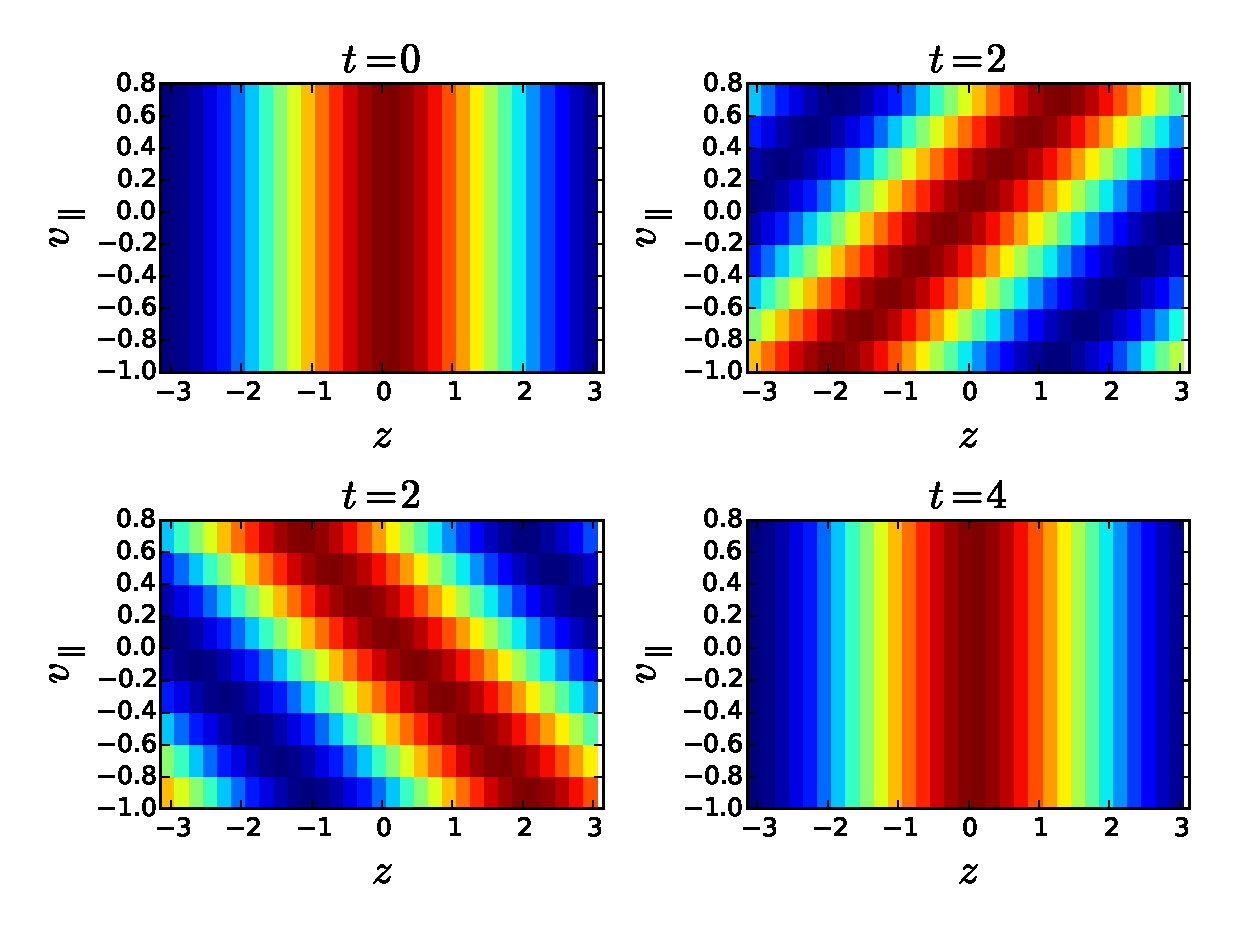
\includegraphics[width=14.8cm]{figs/phmixnl/echo_cartoon.eps}
%    \caption{A cartoon sketch showing how a phase-mixing mode is converted to an
%    phase-unmixing mode. The top left plot shows a phase-mixing mode in the $(z,\vpar)$
%    plane, at time $t=0$ (in
%    arbitrary units) with some parallel structure and no structure in velocity space; this
%    mode then phase-mixes to the one shown in the top right plot at time $t=2$; at which
%    point }
%    \label{phmixnl:fig:echocartoon}
%\end{center}
%\end{figure}
%
There are three separate physical effects manifest in \eqref{phmixnl:eq:gpm}: 
\begin{inparaenum}[(i)]
\item phase mixing/unmixing---the left hand side of \eqref{phmixnl:eq:gpm} is an advection equation in $m$, where
$``+"$ (phase-mixing) modes propagate from small $m$ to large,
and $``-"$ (phase-unmixing) modes propagate from large $m$ back to small; 
\item turbulent cascade---the first term on the right hand side describes nonlinear
coupling of modes with different wavenumbers, which generates fluctuations at small spatial scales;
\item plasma echo---the second term on the right hand side couples the phase-mixing and
phase-unmixing components via nonlinear interaction with the drift velocity. This allows
for a phase-mixing mode propagating to large $m$ to be converted to an phase-unmixing
mode which would propagate back to small $m$, and vice versa.
\end{inparaenum}

In the absence of nonlinear advection ($\Phi = 0$), there is no turbulent cascade, and the
phase-mixing and phase-unmixing
components are decoupled. In this ``linear" limit it can be proven analytically that $\tgm^- = 0$ to lowest
order in $1/\sqrt{m}$, i.e., there is no plasma echo (see \cite{kanekar14a},
\chapref{chap:phmixlin}). Another instance where a
complete lack of an echo can be shown, is when the drift velocity is 2D
($\ppar=0$). Then, the resonance condition $\kpar = \qpar + \ppar = \qpar$ does not allow
$\kpar$ and $\qpar$ to have opposite signs, which according to \eqref{phmixnl:eq:gpm} is a necessary
condition for coupling between phase-mixing and phase-unmixing modes.
Unlike the linear or the 2D drift velocity limit,
a 3D drift velocity ($\ppar\neq0$) has all three aforementioned effects existing
simultaneously in the system.

\subsection{Energetics}
\label{phmixnl:sec:energetics}

In order to understand the relative importance of these three effects, we diagnose how the
free energy of perturbations, $W = \int d
\mb{r} \lt(\int d \vpar \langle g^2 \rangle/2 F_0 + \langle \phi^2 \rangle/2 \alpha
\rt)=\int~d\mb{r}\lt[~\sum_m~|g_m|^2+|g_0|^2~(1+\alpha)\rt]$ gets distributed in the phase
space by the dynamics of the system. $W$ is conserved by \eqsdash{phmixnl:eq:driftkin}{phmixnl:eq:boltz}
in absence of dissipation (see Refs.~\cite{schekochihin08, tome, kanekar14a} and
\secref{intro:sec:krmhd:const}).
Phase mixing transfers $W$ from small $m$ to large, phase unmixing brings it back from
large
$m$ to small. Nonlinear advection cascades $W$ to small spatial scales. 

The contribution of individual Hermite moments to the total free energy $W$, 
is given by
$\Fsk=\sqrt{m}k_\perp~|\tgmk|^2$, where we have changed the Hermite space variable
from $m$ to $s=\sqrt{m}$. At large $s$, $\Fsk$ can be split into the phase-mixing ($\Fsk^+$) and
phase-unmixing components ($\Fsk^-$), where $\Fsk^\pm=\sqrt{m}k_\perp~|\tgmk^\pm|^2$ (see
\eqref{phmixnl:eq:gpm}).
To derive evolution equations for
$\Fsk^\pm$, multiply \eqref{phmixnl:eq:gpm} by
$\sqrt{m}~k_\perp~\tgmk^{\pm \star}$ (the asterisk denotes complex conjugate), to
obtain
\bea
    \pd{\Fsk^\pm}{t} \pm \frac{\lt|\kpar\rt|\vth}{\sqrt{2}} \pd{\Fsk^\pm}{s} + 2 \nu
    s^2 \Fsk^\pm + 2 \eta k_\perp^2 \Fsk^\pm =  
    \textit{Nonlinear terms}.
    \label{phmixnl:eq:Fskpm}
\eea
We can now define the flux of energy from low to high $s$ in the large $s$ limit: 
$\Gsk = \lt|\kpar\rt| \vth \lt(\Fsk^+-\Fsk^-\rt)/\sqrt{2}$. The efficiency of phase mixing is then given by the
normalized flux $\sqrt{2}\Gsk/
|\kpar|\vth\Fsk = (\Fsk^+ - \Fsk^-)/(\Fsk^+ + \Fsk^-)$---phase mixing is completely suppressed when this quantity
is zero, whereas when it is one, the amount of phase mixing is same as that for the linear
system. 
An exact expression for the
flux that is valid at all $s$  can be calculated directly from 
\eqref{phmixnl:eq:tgmk}: $\Gsk~=~\lt|\kpar\rt| \vth \sqrt{(m+1)/2} \, \Re \langle
\tg_{m+1,\mb{k}} \tgmk^\star \rangle$. %

\section{Numerical setup}
    
    We solve \eqsdash{phmixnl:eq:g0}{phmixnl:eq:gmeq} numerically using \Gand.
%    a pseudo-spectral
%    scheme: Hermite moments of the perturbed distribution function are represented using
%    Fourier modes, the nonlinear term is calculated in real space. 
%    Due
%    to the background magnetic field, the system described by \eqsdash{phmixnl:eq:driftkin}{phmixnl:eq:boltz}
%    is anisotropic: the parallel wavelengths of all fluctuations are much longer compared
%    to the perpendicular wavelengths. To facilitate an efficient numerical implementation
%    we normalize the perpendicular spatial co-ordinates $x, y$ and the parallel spatial
%    co-ordinate $z$, to independent arbitrary length scales $\rho$ and $L$, respectively
%    (with the assumption $L \gg \rho$). The drift velocity
%    $\mb{u_\perp}$ is normalized to the thermal velocity $\vth$, time is normalized to
%    $L/\vth$. The Hermite moments of the distribution function are in arbitrary units.
%    The distribution function moments $g_m$ and the electric potential
%    $\phi$ are scaled up by a factor of $L/\rho$ so that all normalized terms are order unity. 
%    %Henceforth, all the quantities quoted in this paper are
    %in these normalized units.
    To simplify the analysis we assume that the distribution function is passive, i.e.,
    the drift velocity $\mb{u_\perp}$ is independent of $g$.
    The velocity $\mb{u}_\perp=\hat{\mb{z}}\times\nabla\Phi$ is
    calculated by solving the Langevin equation $\pdt
    \Phi + \gamma \Phi = \kappa$, where $\gamma >0$ and $\kappa$ is Gaussian white noise ($\langle \kappa(t) \kappa(t')\rangle =
    \epsilon \delta(t-t')$) which drives $\Phi$ with power $\epsilon$; $\gamma$ is chosen
    such that the Kubo number is held constant at one (see \secref{pp0:sec:intro}). The drift velocity
    was restricted to a single scale (all wavenumbers $\mb{p}$ such that $p_\perp=1,
    \ppar=1$), the largest scale in our numerical box.
    The
    saturated root mean square amplitude of the drift velocity can be calculated using the
    fluctuation-dissipation theorem \cite{kubo66}: $\langle u_\perp^2 \rangle
    = p_\perp^2 \epsilon/2 \gamma$. In light of these simplifications, one can estimate
    the turbulent cascade rate as $\tau_C^{-1}\sim \pu$, which we control in our simulations by
    changing $\epsilon$.
    
    The source term in \eqref{phmixnl:eq:g0}, $\chi_0$, is assumed to be delta-correlated
    in time, and
    $\chi_1$ is set to zero. Since \eqref{phmixnl:eq:driftkin} is
    homogeneous in $g$, the power with which $\chi_0$ injects energy into the system can
    be set to unity without loss of generality.

    Instead of using the Lenard-Bernstein collision operator or
    regular viscosity as in \eqref{phmixnl:eq:gmeq}, we use hypercollisions ($-\nu m^8 g_m$)
    and hyperviscosity ($-\eta k_\perp^8 g_m$) to efficiently utilize
    computational resources. The dissipation microscales for these operators can be estimated
    as $s_c = \sqrt{m_c} = \lt(\ppar \vth/\nu\rt)^{1/17}$ and $k_{\perp, \eta} = \lt(
    |u_\perp|/\eta \rt)^{1/8}$, where $s_c$ is the collisional cutoff for modes with
    parallel wavenumber $\ppar$; $k_{\perp,
    \eta}$ is the viscous cutoff. A simulation is fully characterized by 3 parameters:
    the nonlinear advection rate $\tau_C^{-1}$, the collisional cutoff $s_c$ and the viscous
    cutoff $k_{\perp, \eta}$.  
    All the results included in this chapter are from a simulation with parameters $\tau_C
    \simeq 1.5$, $s_c \simeq 21.3$ and $k_{\perp, \eta} \simeq 18.8$.

\section{Results}
    \subsection{Phase mixing efficiency}

    \begin{figure}
    \begin{center}
        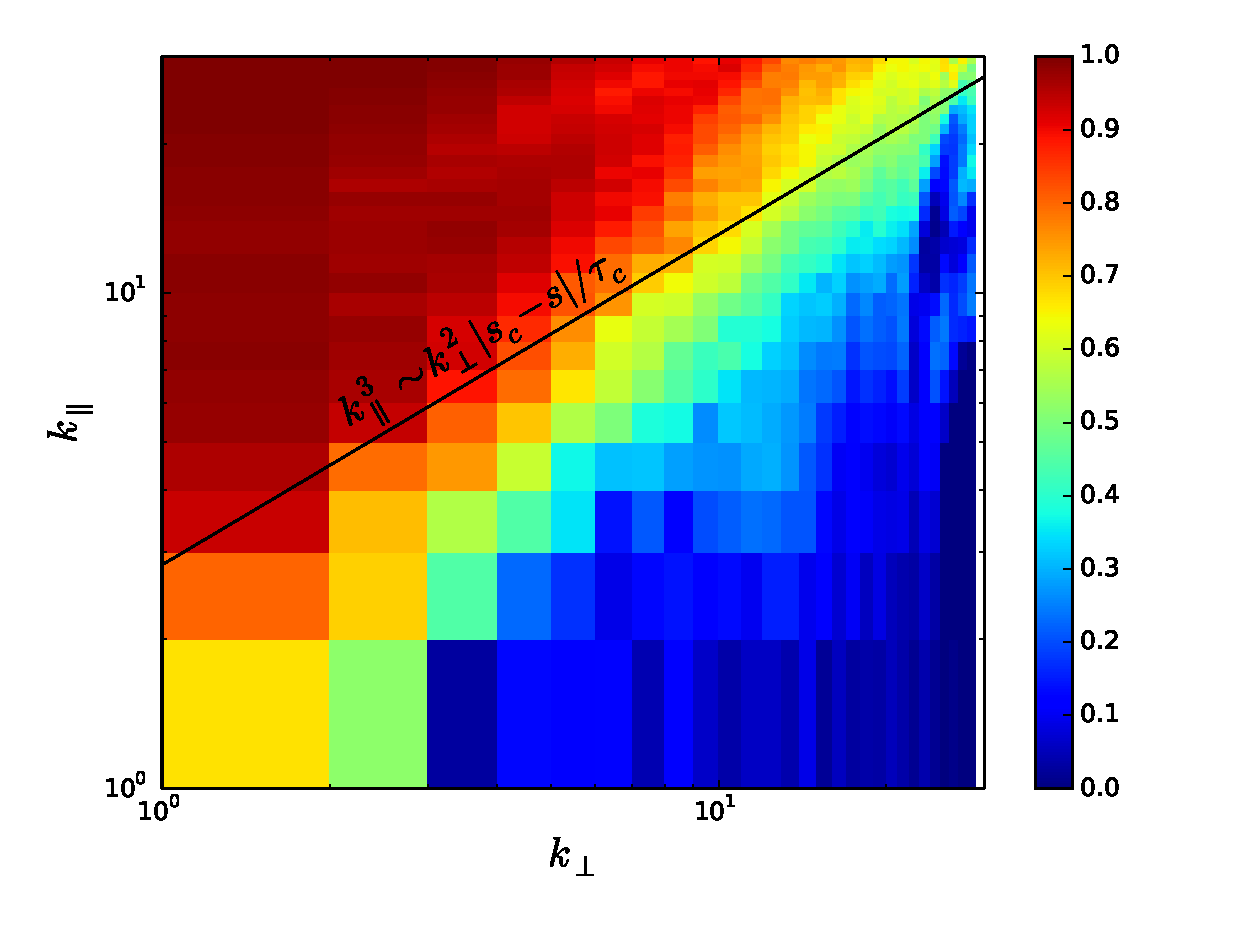
\includegraphics[width=14.8cm]{figs/phmixnl/M900_m100_pmsupp_vskpkz.eps}
        \caption{Normalized flux (defined after \eqref{phmixnl:eq:Fskpm}) through $s=10$ vs
        $k_\perp-\kpar$. Phase mixing is nearly completely suppressed for $\kpar^3 \leq
        k_\perp^2 \lt|s_c -s\rt|/\tau_C$.}
        \label{phmixnl:fig:m100supp:vskpkz}
    \end{center}
    \end{figure}
    \begin{figure}
    \begin{center}
        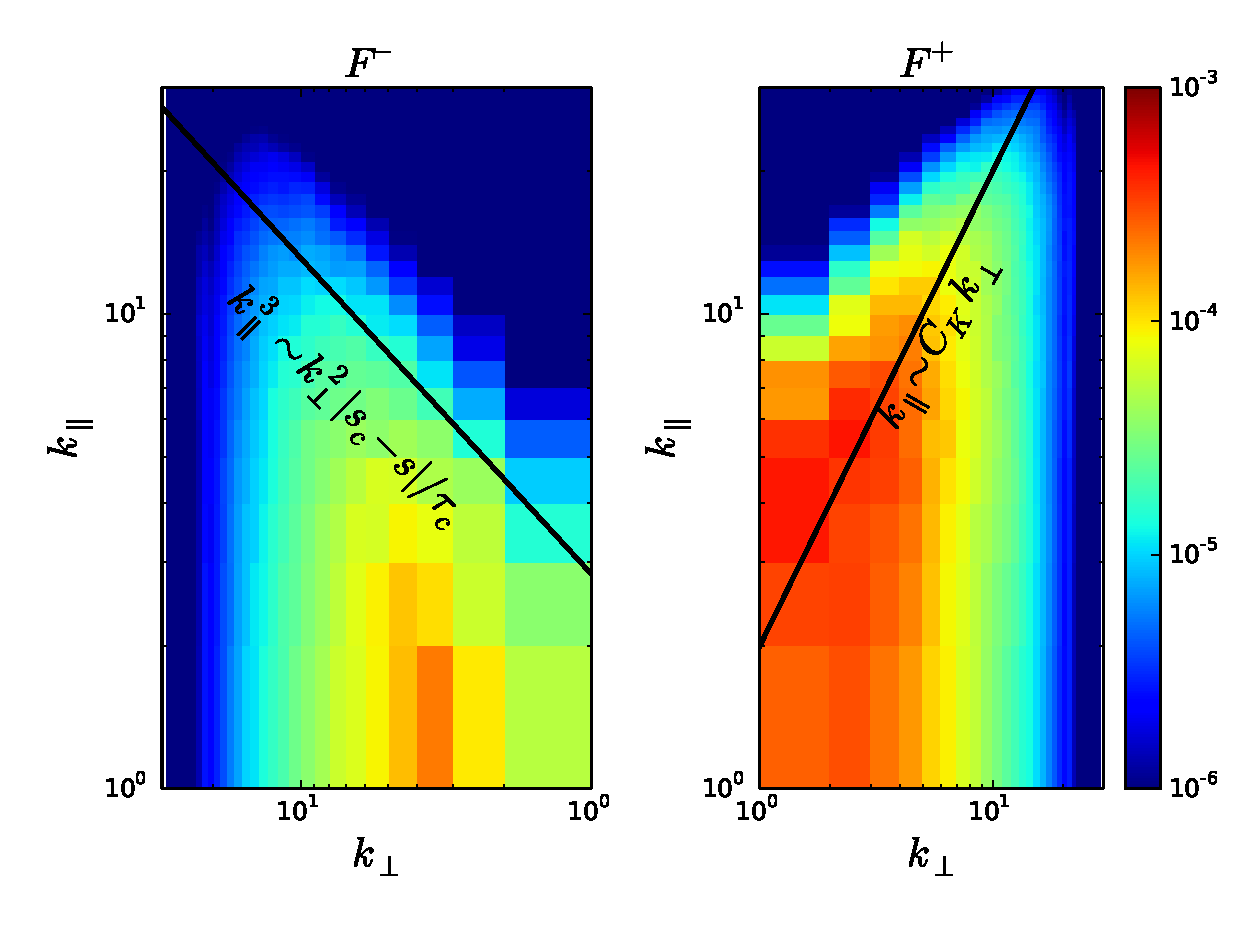
\includegraphics[width=14.8cm]{figs/phmixnl/M900_m100_fpm_vskpkz.eps}
        \caption{$\Fsk^\pm$ (defined before \eqref{phmixnl:eq:gpm}) at $s=10$ vs
        $k_\perp-\kpar$; $F^-$ is plotted on the left, $F^+$ on the right. The horizontal
        axis for $F^-$ is reversed, so as to facilitate comparison with the $F^+$
        plot. For $\kpar^3 \geq k_\perp^2 \lt|s_c-s\rt|/\tau_C$,
        there is negligible $\Fsk^-$. $\Fsk^+$ is seen to cascade to large wavenumbers
        along the $\kpar\sim C_K k_\perp$ line.}
        \label{phmixnl:fig:m100fpm:vskpkz}
    \end{center}
    \end{figure}

    \begin{figure}
    \begin{center}
        \includegraphics[width=14.8cm]{figs/phmixnl/M900_m100_pmsupp_vsskz.eps}
        \caption{Normalized flux (defined after \eqref{phmixnl:eq:Fskpm}) at $k_\perp=8$ vs
        $\kpar-s$. Phase mixing is nearly completely suppressed for $\kpar^3 \leq
        k_\perp^2 \lt|s_c -s\rt|/\tau_C$.}
        \label{phmixnl:fig:m100supp:vsskz}
    \end{center}
    \end{figure}
    \begin{figure}
    \begin{center}
        \includegraphics[width=14.8cm]{figs/phmixnl/M900_m100_fpm_vsskz.eps}
        \caption{$\Fsk^\pm$ (defined before \eqref{phmixnl:eq:gpm}) at $k_\perp=8$ vs
        $\kpar-s$; $F^-$ is plotted on the left, $F^+$ on the right. The horizontal
        axis for $F^-$ is reversed, so as to facilitate comparison with the $F^+$
        plot. For $\kpar^3 \geq k_\perp^2 \lt|s_c-s\rt|/\tau_C$,
        there is negligible $\Fsk^-$.}
        \label{phmixnl:fig:m100fpm:vsskz}
    \end{center}
    \end{figure}

    \begin{figure}
    \begin{center}
        \includegraphics[width=14.8cm]{figs/phmixnl/M900_m100_pmsupp_vsskp.eps}
        \caption{Normalized flux (defined after \eqref{phmixnl:eq:Fskpm}) at $\kpar=8$ vs
        $k_\perp-s$. Phase mixing is nearly completely suppressed for $\kpar^3 \leq
        k_\perp^2 \lt|s_c -s\rt|/\tau_C$.}
        \label{phmixnl:fig:m100supp:vsskp}
    \end{center}
    \end{figure}
    \begin{figure}
    \begin{center}
        \includegraphics[width=14.8cm]{figs/phmixnl/M900_m100_fpm_vsskp.eps}
        \caption{$\Fsk^\pm$ (defined before \eqref{phmixnl:eq:gpm}) at $\kpar=8$ vs
        $k_\perp-s$; $F^-$ is plotted on the left, $F^+$ on the right. The horizontal
        axis for $F^-$ is reversed, so as to facilitate comparison with the $F^+$
        plot. For $\kpar^3 \geq k_\perp^2 \lt|s_c-s\rt|/\tau_C$,
        there is negligible $\Fsk^-$.}
        \label{phmixnl:fig:m100fpm:vsskp}
    \end{center}
    \end{figure}

    Since we chose the drift velocity to be a single scale velocity field with $\ppar=1$,
    the nonlinear term couples modes whose parallel wavenumbers differ from each other by
    one. A phase mixing mode at $s=1$, with a parallel wavenumber $\kpar$, is converted to
    an phase-unmixing mode only if the two have oppositely signed parallel wavenumbers
    (see \eqref{phmixnl:eq:gpm}). Hence, such a phase-mixing mode has to go through at least
    $\kpar$ nonlinear interactions in order to reach $\kpar=0$, before it can be
    converted to an phase-unmixing mode.
    While this phase-mixing mode cascades to
    $\kpar=0$, it also gets transferred to a larger $s$ due to phase mixing. If this value
    of $s$
    is comparable to the collisional cutoff $s_c$, a part of the energy is lost to
    collisions, and only the remaining energy gets converted to an phase-unmixing mode---this sets a bound on the extent of the plasma echo in the phase space. 
    We observe in our simulations that the plasma echo is restricted to the $\kpar^3 \leq
    k_\perp^2 \lt|s_c-s\rt|/\tau_C$ region of the phase space as seen in
    \figsdash{phmixnl:fig:m100supp:vskpkz}{phmixnl:fig:m100fpm:vsskp}.
    As a result of the echo, phase mixing is significantly suppressed for $\kpar^3~\leq~k_\perp^2 \lt|s_c-s\rt|/\tau_C$. 

\subsection{Spectra vs $(s, k_\perp, \kpar)$}

    \begin{figure}
    \begin{center}
        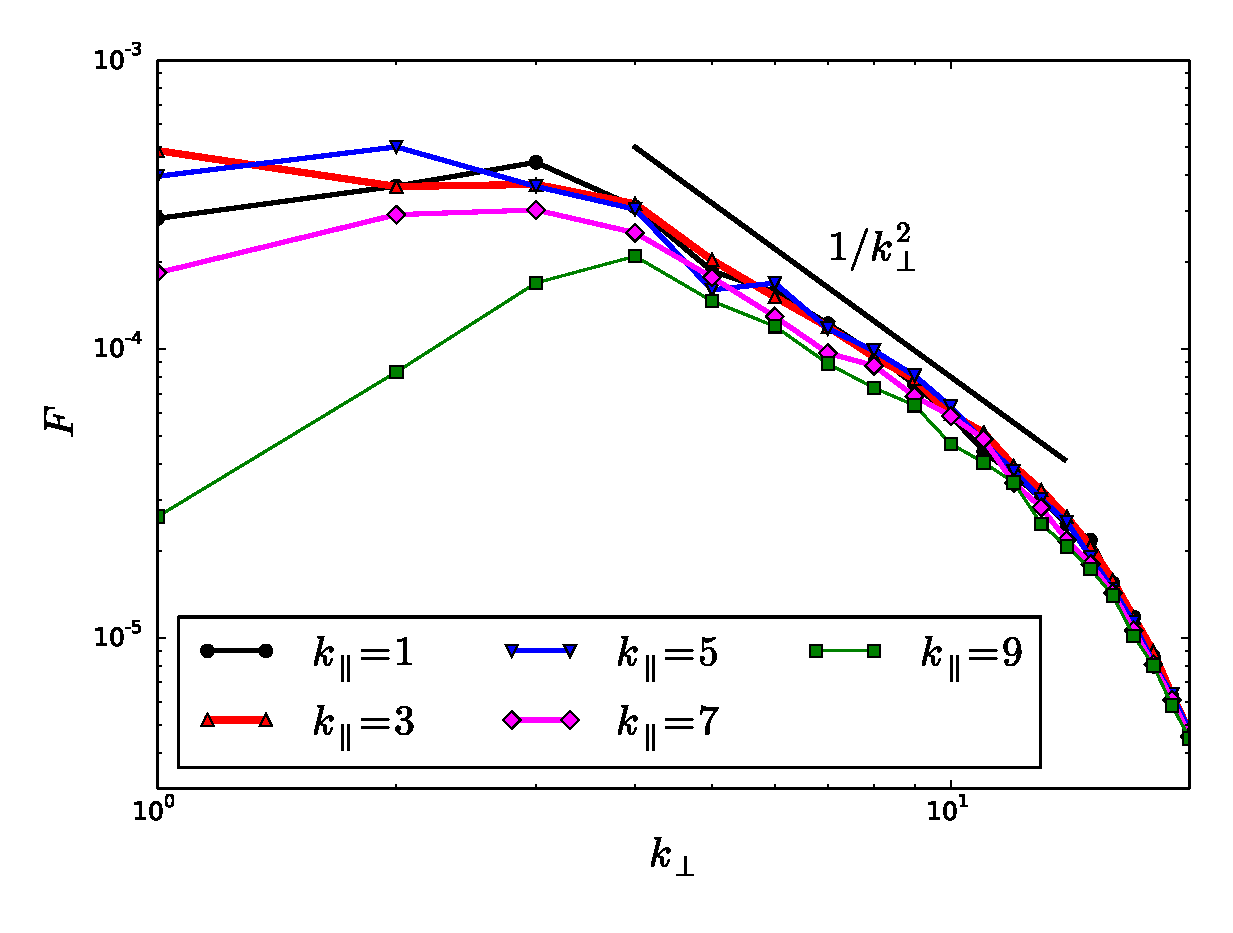
\includegraphics[width=14.8cm]{figs/phmixnl/M900_m100_vskp.eps}
        \caption{$\Fsk$ vs $k_\perp$ for $s=10$. $\Fsk$ increases for $k_\perp \leq \kpar/C_K$, and
        then is $\sim 1/k_\perp^2$.}
        \label{phmixnl:fig:m100f:vskp}
    \end{center}
    \end{figure}
    \begin{figure}
    \begin{center}
        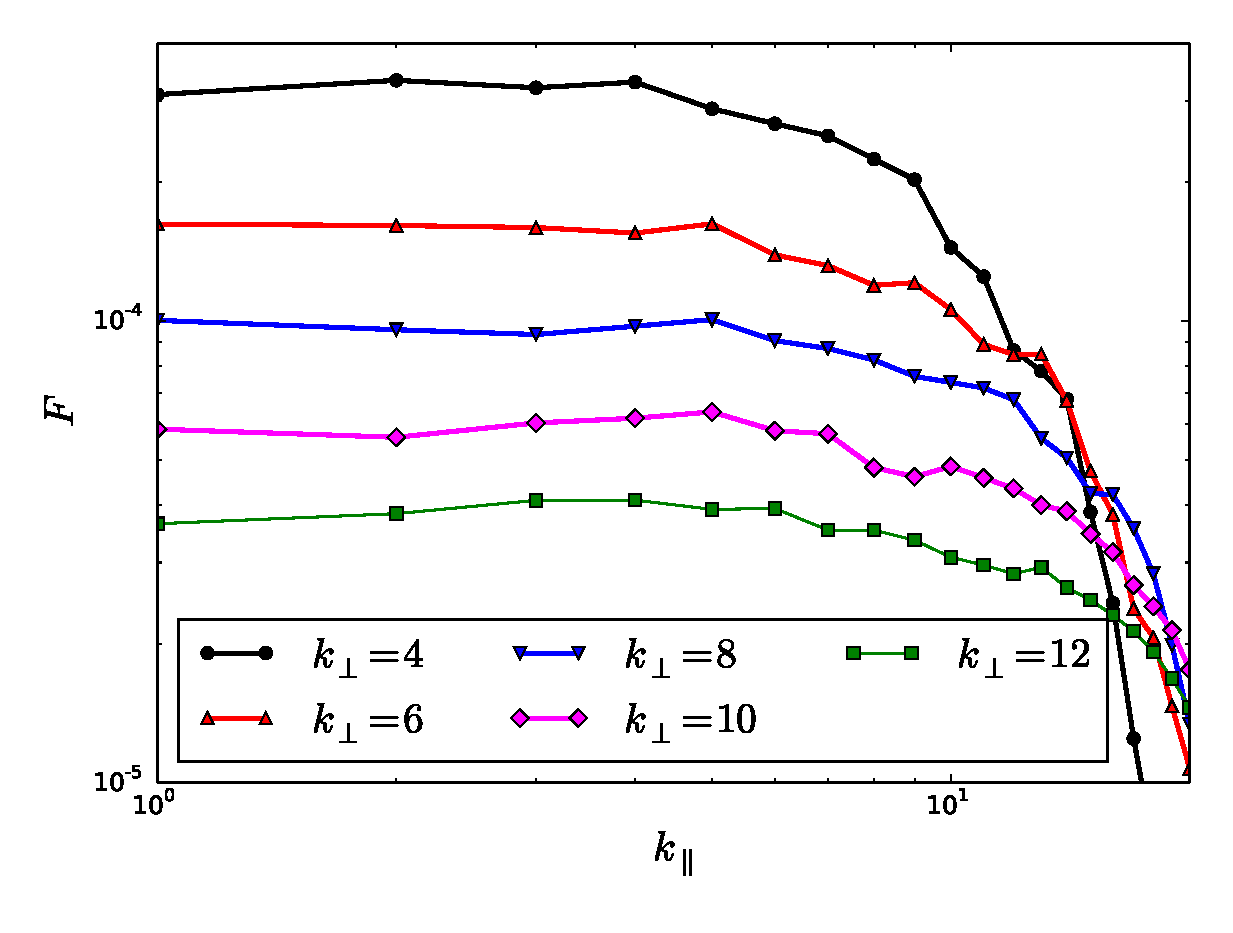
\includegraphics[width=14.8cm]{figs/phmixnl/M900_m100_vskz.eps}
        \caption{$\Fsk$ vs $\kpar$ for $s=10$. $\Fsk$ is a constant $\kpar \leq C_K k_\perp$, and
        then steeply rolls off.}
        \label{phmixnl:fig:m100f:vskz}
    \end{center}
    \end{figure}

   In the previous section we saw that the phase space is split into a suppressed and an
   unsuppressed region by the $\kpar^3 \sim k_\perp^2 \lt|s_c-s\rt|/\tau_C$ line. In this
   section we discuss how the spectra look like in the $(s, k_\perp, \kpar)$ phase space. 

    From \figref{phmixnl:fig:m100fpm:vskpkz}, we
    see that the phase-mixing component cascades to small spatial scales along the $\kpar
    \sim C_K k_\perp$ line\footnote{This may be thought of as the analog of a
    critical-balance style relationship between parallel and perpendicular wavenumbers in
    our model; $C_K$ is the equivalent Kolmogorov-constant.}, where $C_K$ is a constant (we observe $C_K\approx 2$). This
    relationship between the parallel and the perpendicular wavenumber can also be seen
    from the 1D spectra plotted in \figsand{phmixnl:fig:m100f:vskp}{phmixnl:fig:m100f:vskz}: the perpendicular
    spectra increase till $k_\perp \leq \kpar/C_K$, and then are approximately $\sim 1/k_\perp^2$,
    whereas the parallel spectra are constant till $\kpar \leq C_K k_\perp$ and then roll
    off steeply.

    In order to understand these spectra, we add the $``+"$ and $``-"$ equations in
    \eqref{phmixnl:eq:Fskpm}, to derive an equation for the spectrum $\Fsk$:
    \bea
        \pd{\Fsk}{t} + \pd{\Gsk}{s} + 2 \nu
        s^2 \Fsk + 2 \eta k_\perp^2 \Fsk =  
        \textit{Nonlinear terms}.
        \label{phmixnl:eq:Fsk}
    \eea
    For the suppressed region of the phase space, $\Gsk \approx 0$, i.e., the steady state
    spectrum is a zero flux solution. Setting $\Gsk=0$ in \eqref{phmixnl:eq:Fsk}
    reduces the problem to the fluid limit. It can be shown in this limit that the spectrum is given by $\Fsk
    \propto k_\perp/\lt(\kpar^2 + C_K^2 k_\perp^2\rt)^{3/2}$; this is consistent with the
    spectra observed in \figsand{phmixnl:fig:m100f:vskp}{phmixnl:fig:m100f:vskz}. 

    \begin{figure}
    \begin{center}
        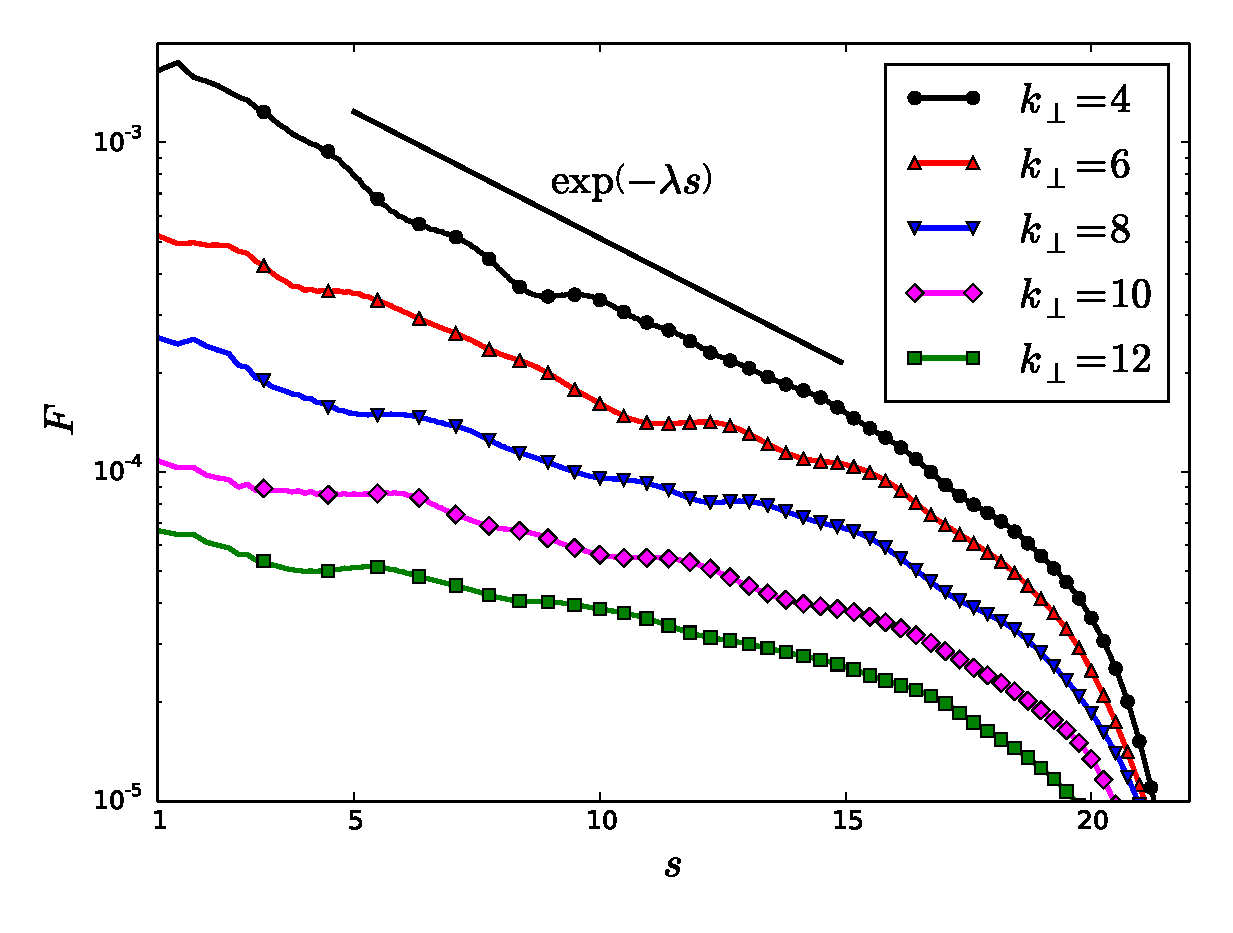
\includegraphics[width=14.8cm]{figs/phmixnl/M900_kz2_vss.eps}
        \caption{$\Fsk$ vs $s$ for $\kpar=2$. The spectrum decays in $s$ at a rate $\lambda \propto
        1/k_\perp$ (see \figref{phmixnl:fig:lambda:vskp}) in the region where phase-mixing is
        suppressed (see
        \figsdash{phmixnl:fig:m100supp:vskpkz}{phmixnl:fig:m100fpm:vsskp}).}
        \label{phmixnl:fig:m100f:kz2:vss}
    \end{center}
    \end{figure}
    \begin{figure}
    \begin{center}
        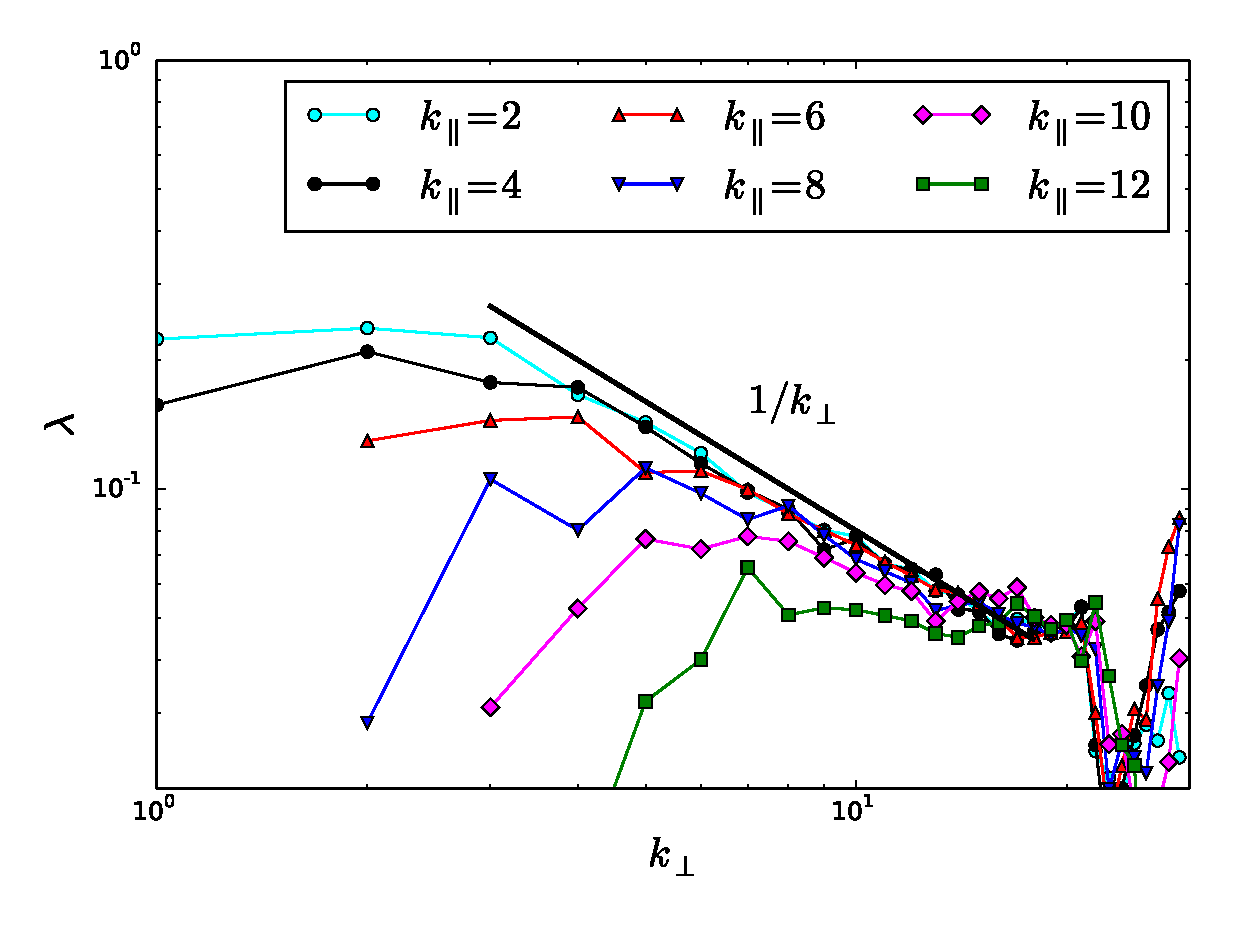
\includegraphics[width=14.8cm]{figs/phmixnl/M900_lambda_vskp.eps}
        \caption{The rate $\lambda$ at which spectrum $\Fsk$ decays in $s$ (see
        \figref{phmixnl:fig:m100f:kz2:vss}) vs $k_\perp$. We observe that $\lambda \propto
        1/k_\perp$ in the suppressed region; in the unsuppressed region $\lambda \approx
        0$.}
        \label{phmixnl:fig:lambda:vskp}
    \end{center}
    \end{figure}
    \begin{figure}
    \begin{center}
        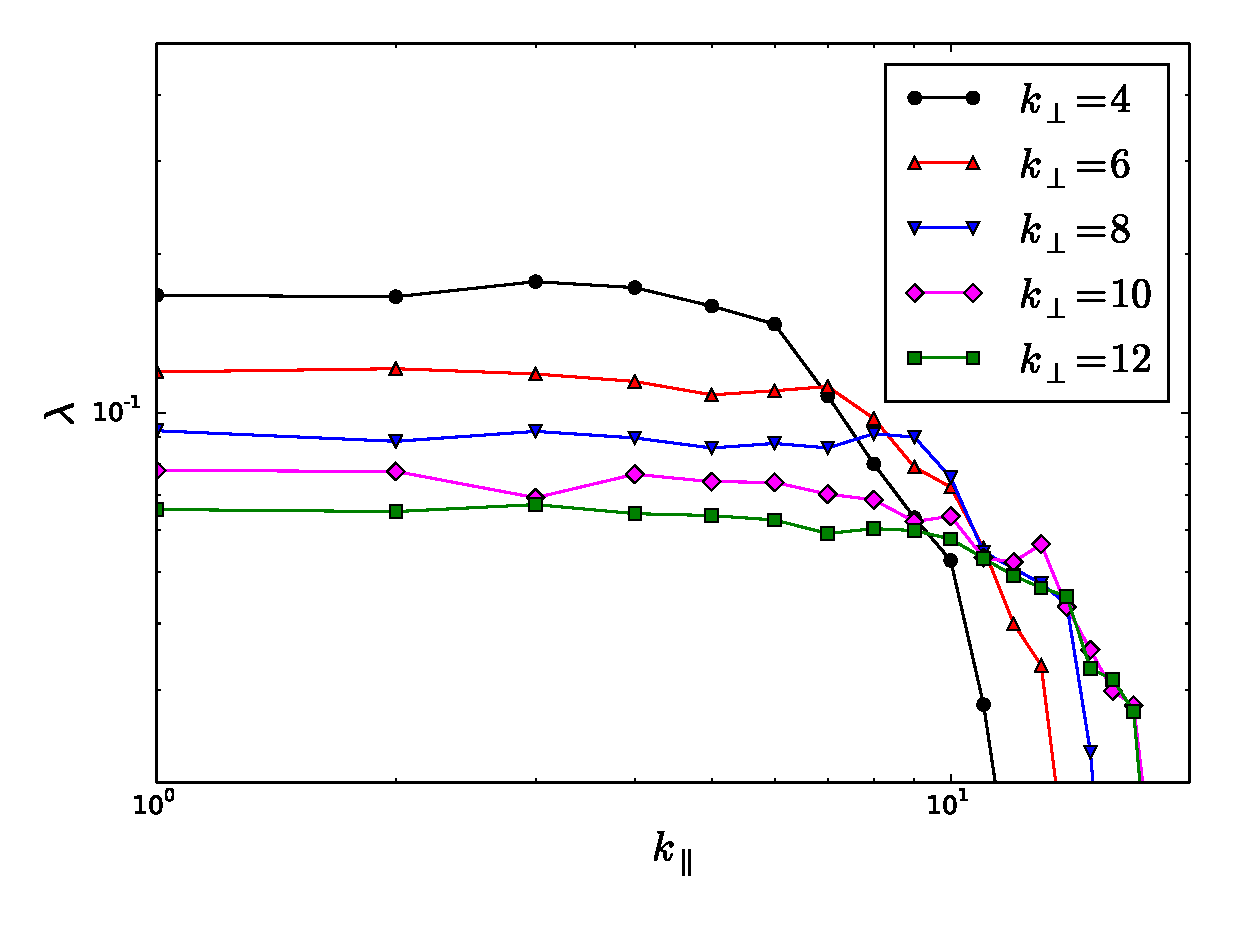
\includegraphics[width=14.8cm]{figs/phmixnl/M900_lambda_vskz.eps}
        \caption{The rate $\lambda$ at which spectrum $\Fsk$ decays in $s$ (see
        \figref{phmixnl:fig:m100f:kz2:vss}) vs $\kpar$. $\lambda$ is independent of $\kpar$ in the
        suppressed region; in the suppressed region $\lambda \to 0$.}
        \label{phmixnl:fig:lambda:vskz}
    \end{center}
    \end{figure}
    \begin{figure}
    \begin{center}
        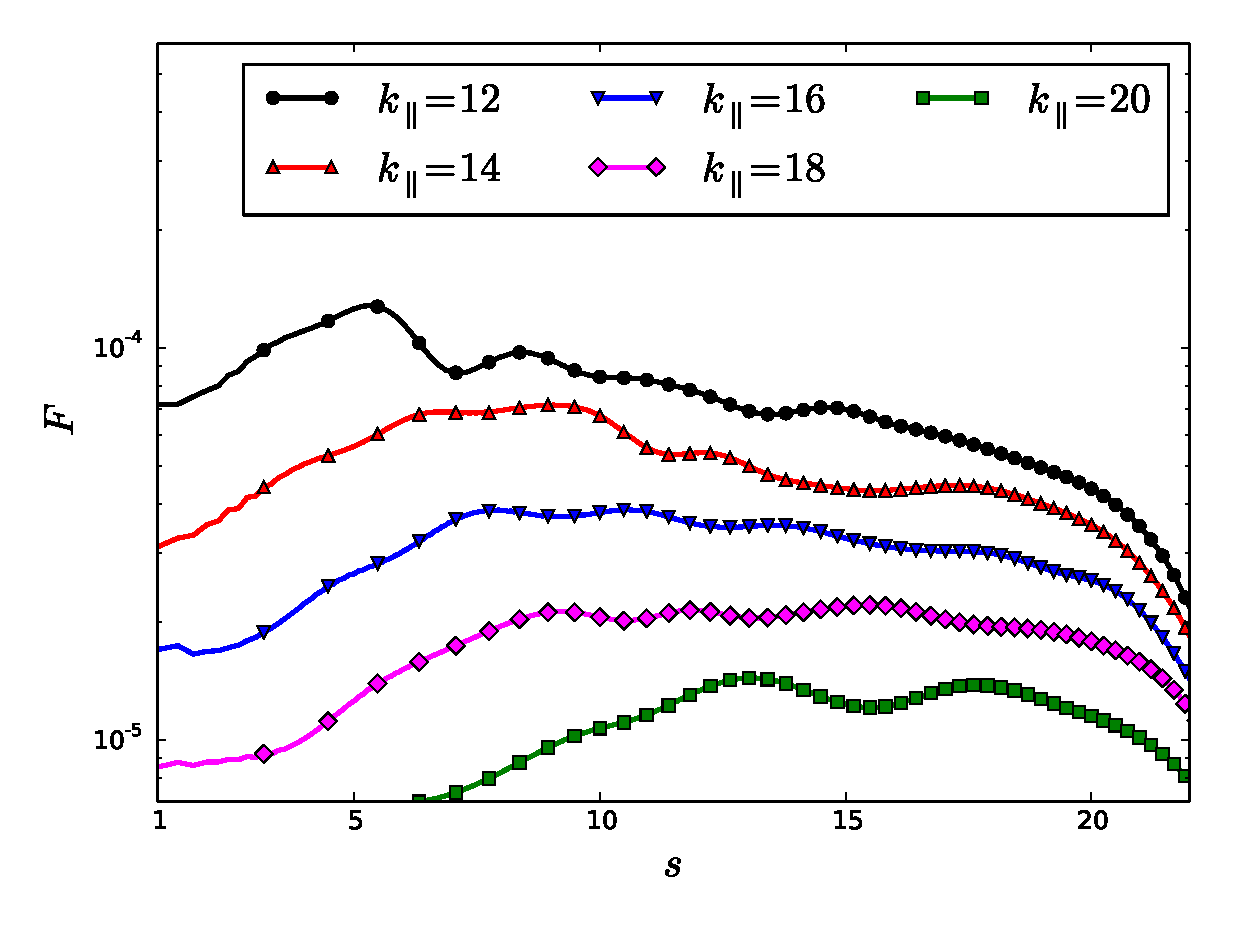
\includegraphics[width=14.8cm]{figs/phmixnl/M900_kp6_vss.eps}
        \caption{$\Fsk$ vs $s$ for $k_\perp=6$. In the unsuppressed region the
        spectrum vs $s$ is constant.}
        \label{phmixnl:fig:m100f:kp6:vss}
    \end{center}
    \end{figure}
    
    The spectra versus $s$ in the suppressed region are observed to decay exponentially 
     at a rate proportional to 
    $1/k_\perp$, and independent of $\kpar$ (see
    \figsref{phmixnl:fig:m100f:kz2:vss}{phmixnl:fig:lambda:vskp}{phmixnl:fig:lambda:vskz}).
    In the unsuppressed (phase-mixed) region, the $s$ spectrum is constant (see
    \figsref{phmixnl:fig:lambda:vskp}{phmixnl:fig:lambda:vskz}{phmixnl:fig:m100f:kp6:vss}), which is the
    same spectrum as that for the Landau-damped solution\footnote{Since the spectrum
    plotted in this chapter is $\Fsk=\sqrt{m}k_\perp|\tgmk|^2$, a constant-in-$s$ spectrum
    is same as the $|g_m|^2 \sim 1/\sqrt{m}$ spectrum from \chapref{chap:phmixlin}.} \cite{watanabe04, zocco11,
    hatch13, kanekar14a}.

%\subsection{$s=1$}
%    \begin{figure}
%    \begin{center}
%        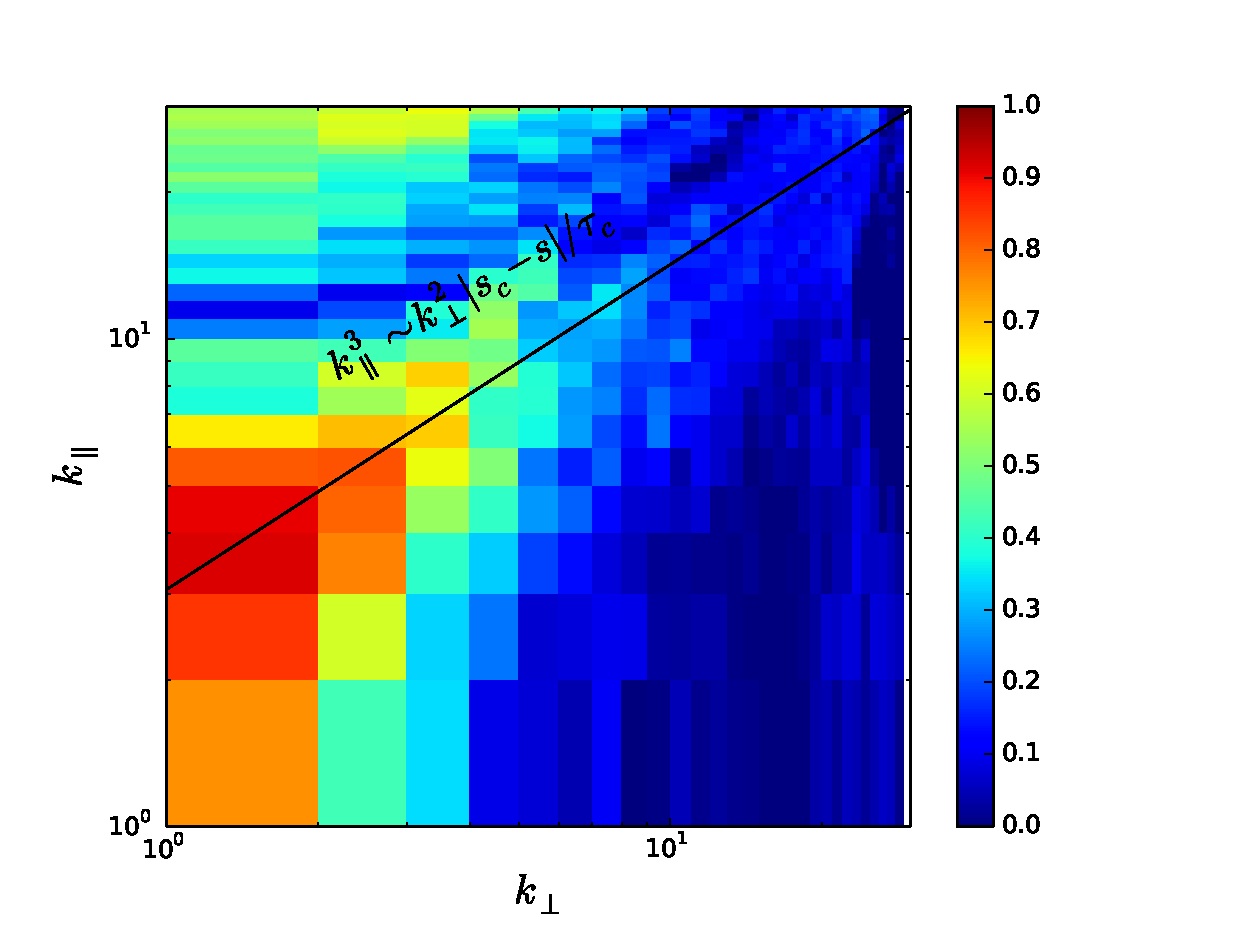
\includegraphics[width=14.8cm]{figs/phmixnl/M900_m1_exsupp_vskpkz.eps}
%        \caption{Exact normalized flux through $s=1$ vs $k_\perp-\kpar$}
%    \end{center}
%    \end{figure}
%    \begin{figure}
%    \begin{center}
%        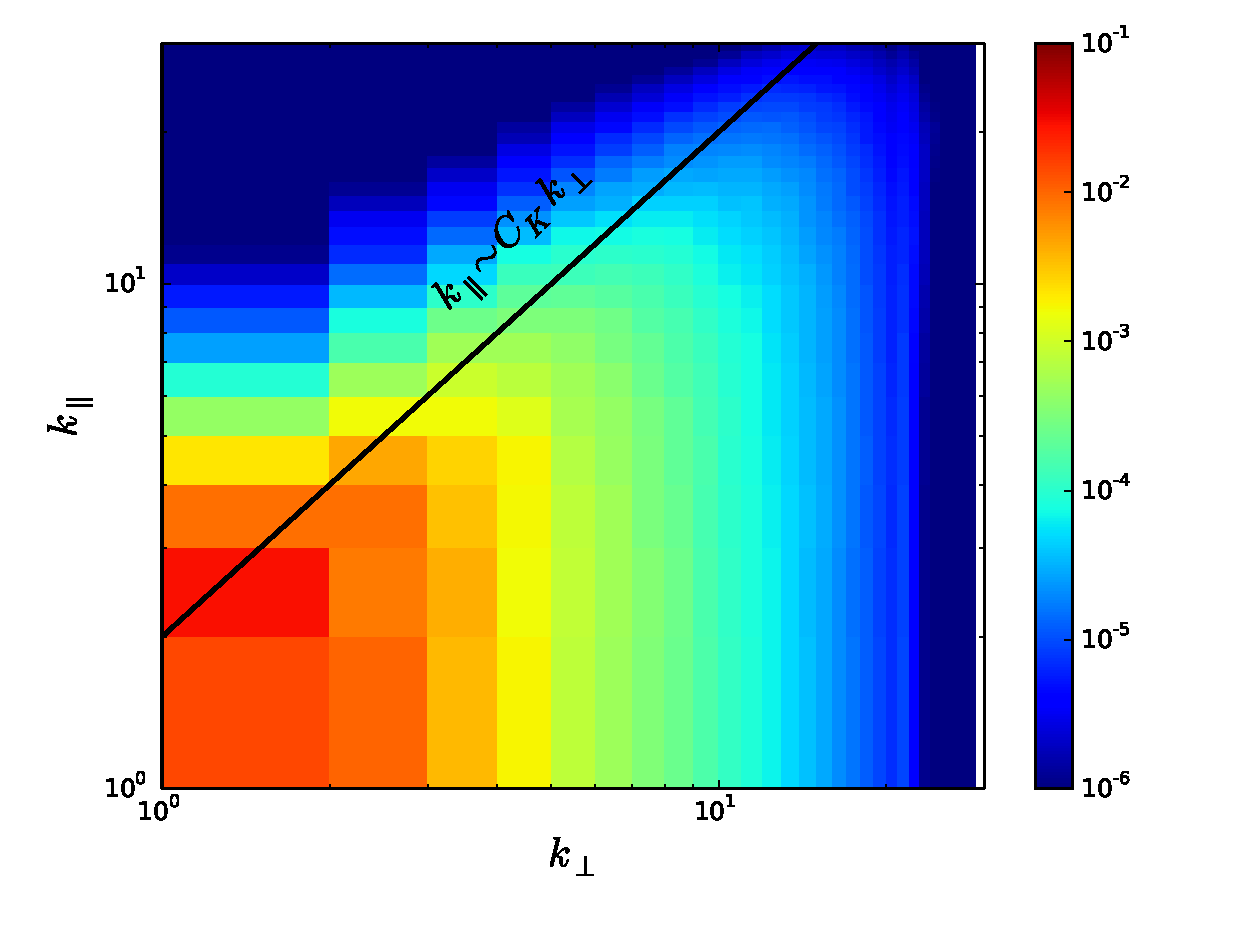
\includegraphics[width=14.8cm]{figs/phmixnl/M900_m1_f_vskpkz.eps}
%    \end{center}
%    \end{figure}
%    \begin{figure}
%    \begin{center}
%        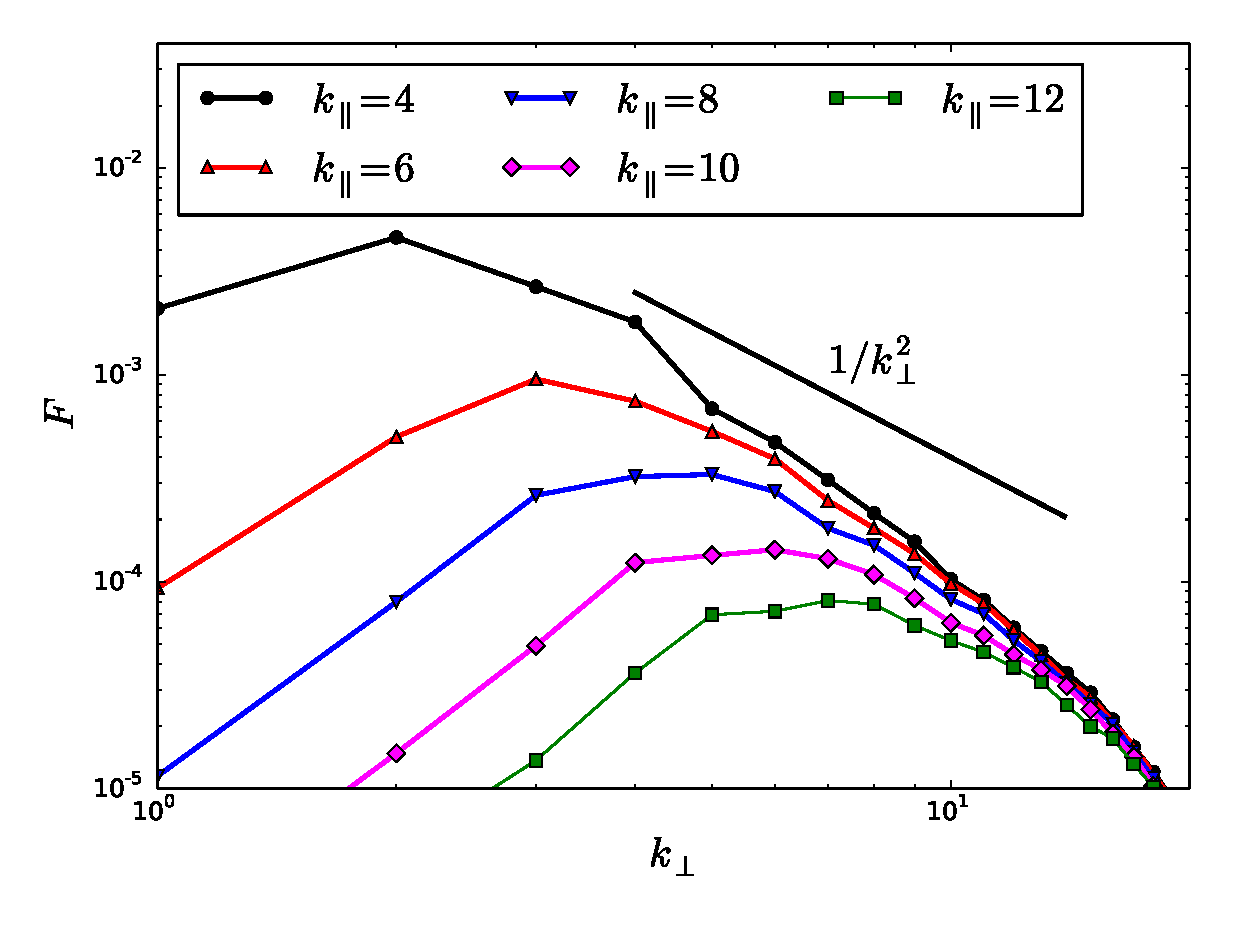
\includegraphics[width=14.8cm]{figs/phmixnl/M900_m1_vskp.eps}
%    \end{center}
%    \end{figure}
%    \begin{figure}
%    \begin{center}
%        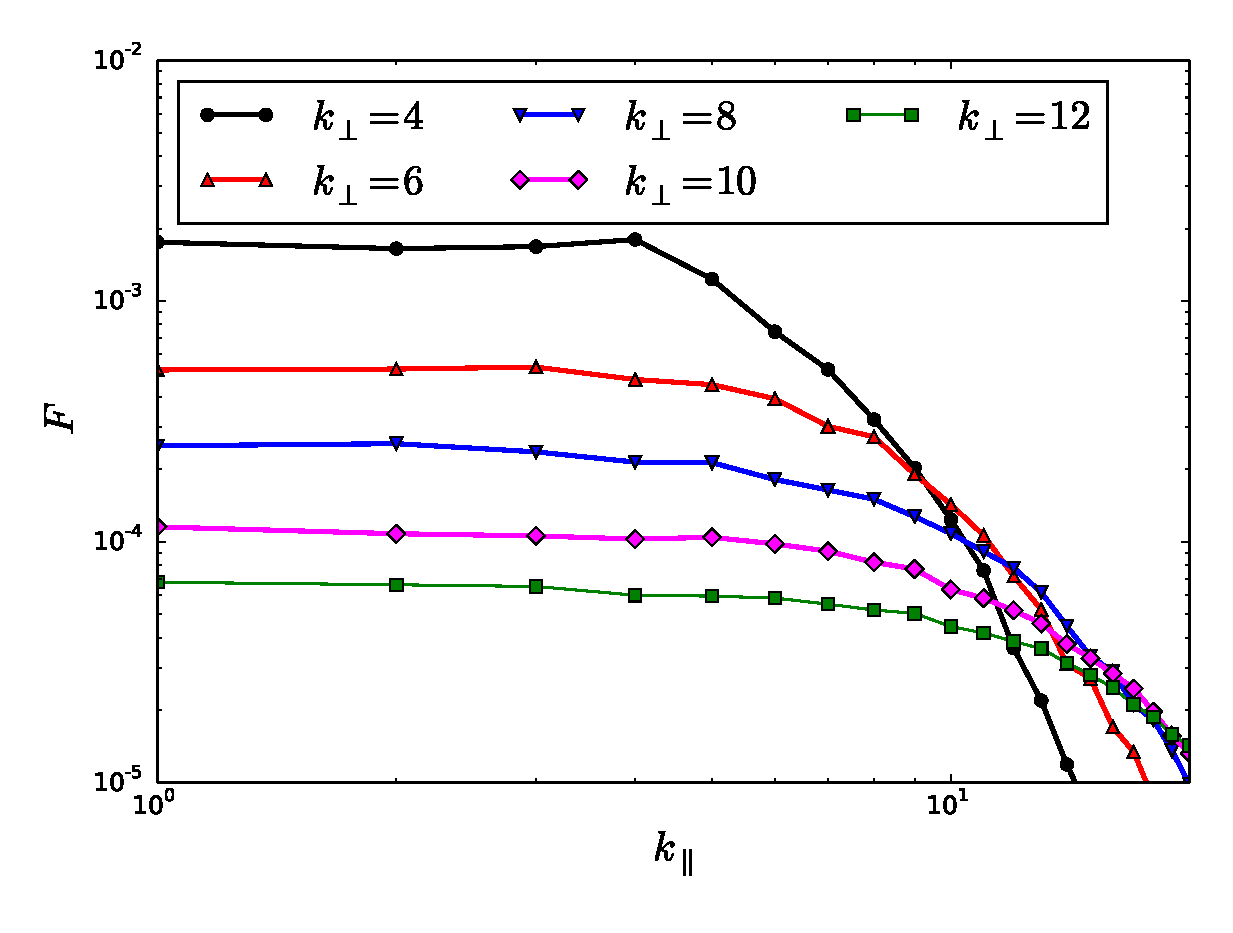
\includegraphics[width=14.8cm]{figs/phmixnl/M900_m1_vskz.eps}
%    \end{center}
%    \end{figure}
%    
%    \begin{figure}
%    \begin{center}
%        \includegraphics[width=14.8cm]{figs/phmixnl/M900_m1_vskpkz.eps}
%        \caption{Spectrum $\Fsk$ vs $k_\perp, \kpar$ at $s=1$ for parameters $\tauc
%        \simeq 1.5$, $s_c \simeq 17.5$, $k_{\perp, \eta} = 17.4$. The energy cascade proceeds
%        along the $\kpar \sim C_K k_\perp$ line; most of the energy is contained within
%        the cone below this line ($\kpar \leq C_K k_\perp$).}
%        \label{phmixnl:fig:kpkzspec}
%    \end{center}
%    \end{figure}
%    \begin{figure}
%    \begin{center}
%        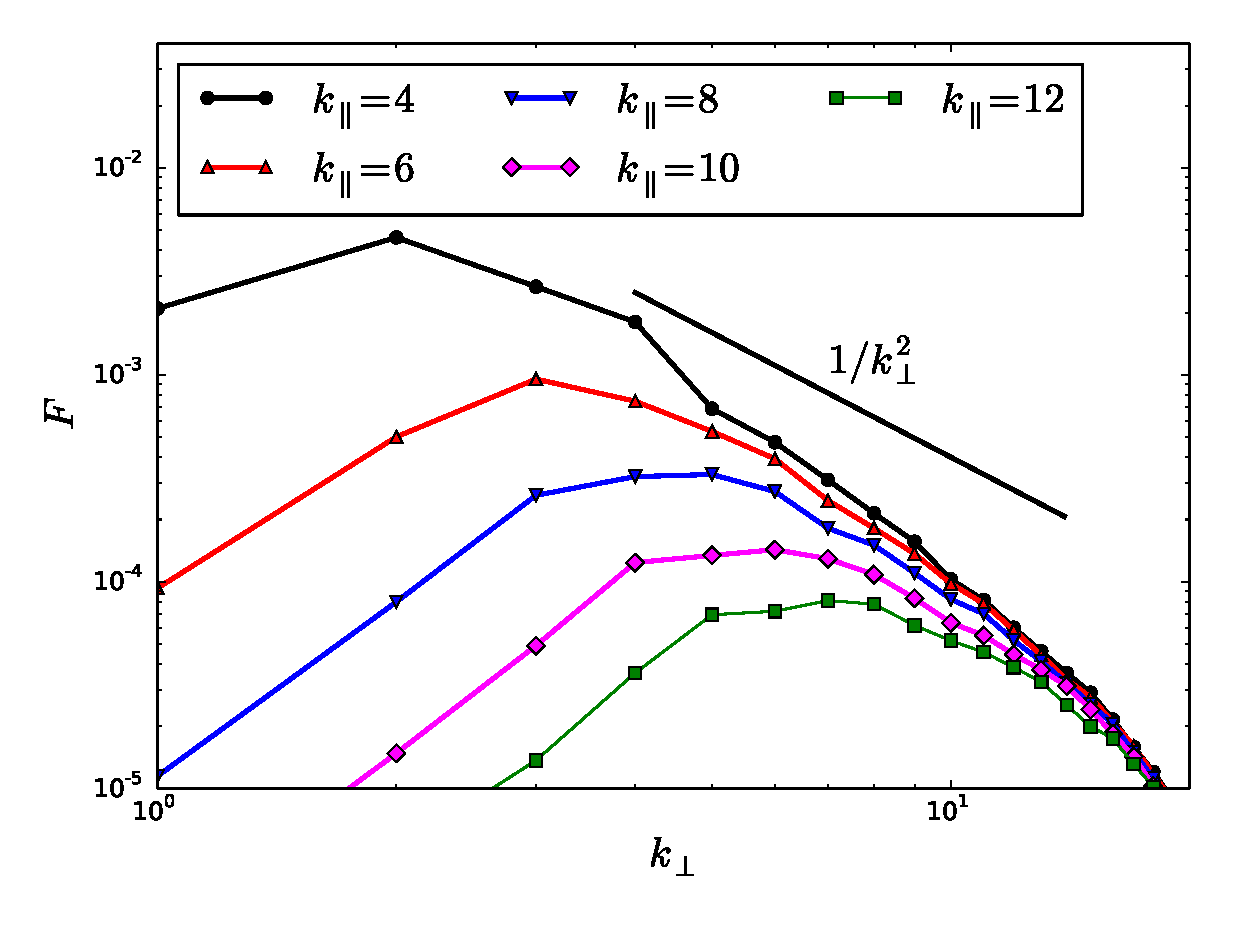
\includegraphics[width=14.8cm]{figs/phmixnl/M900_m1_vskp.eps}
%        \caption{Perpendicular spectrum at $s=1$ for parameters $\tauc
%        \simeq 1.5$, $s_c \simeq 17.5$, $k_{\perp, \eta} = 17.4$. For $\kpar \leq C_K
%        k_\perp$ the spectrum is $\sim 1/k_\perp^2$.} 
%        \label{phmixnl:fig:1dkpspec}
%    \end{center}
%    \end{figure}
%    \begin{figure}
%    \begin{center}
%        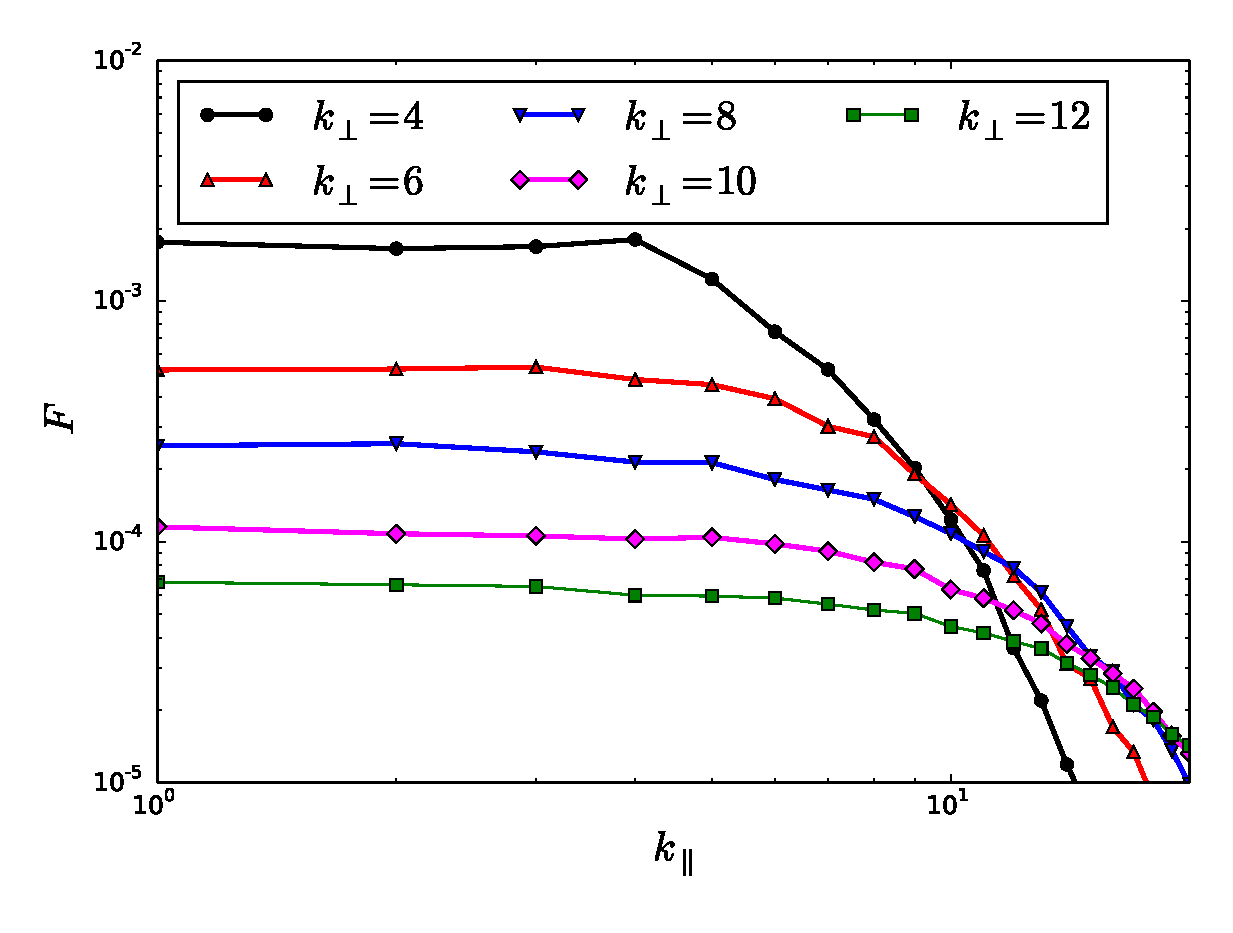
\includegraphics[width=14.8cm]{figs/phmixnl/M900_m1_vskz.eps}
%        \caption{Parallel spectrum at $s=1$ for parameters $\tauc
%        \simeq 1.5$, $s_c \simeq 17.5$, $k_{\perp, \eta} = 17.4$. For $\kpar \leq C_K
%        k_\perp$ the parallel spectrum is constant.}
%        \label{phmixnl:fig:1dkzspec}
%    \end{center}
%    \end{figure}
%
%    The cascade in real space is observed to proceed along the
%    $\kpar\sim~C_K~k_\perp$ line (see
%    \figref{phmixnl:fig:kpkzspec}), where $C_K$ is a constant that relates the parallel and
%    perpendicular wavenumbers \footnote{Scaling argument}; in our simulations we observe $C_K \approx 2$.  
%    Most of the energy in the system is contained within the
%    $\kpar \leq C_K k_\perp$ region. The relationship between the parallel and
%    perpendicular wavenumbers can also be seen from 1D spectra shown in
%    \figsand{phmixnl:fig:1dkpspec}{phmixnl:fig:1dkzspec}. The perpendicular spectrum at a fixed parallel
%    wavenumber $\kpar$ increases till $k_\perp \leq \kpar/C_K$, beyond which it goes as
%    $1/k_\perp^2$. The parallel spectrum at a fixed wavenumber $k_\perp$ remains constant
%    till $\kpar \leq C_K k_\perp$, and falls off rapidly for larger parallel wavenumbers.
%    These 1D spectra reaffirm the assertion that $\kpar \leq C_K k_\perp$ is the
%    energetically relevant region of the phase space for our model.
%
%    \begin{figure}
%    \begin{center}
%        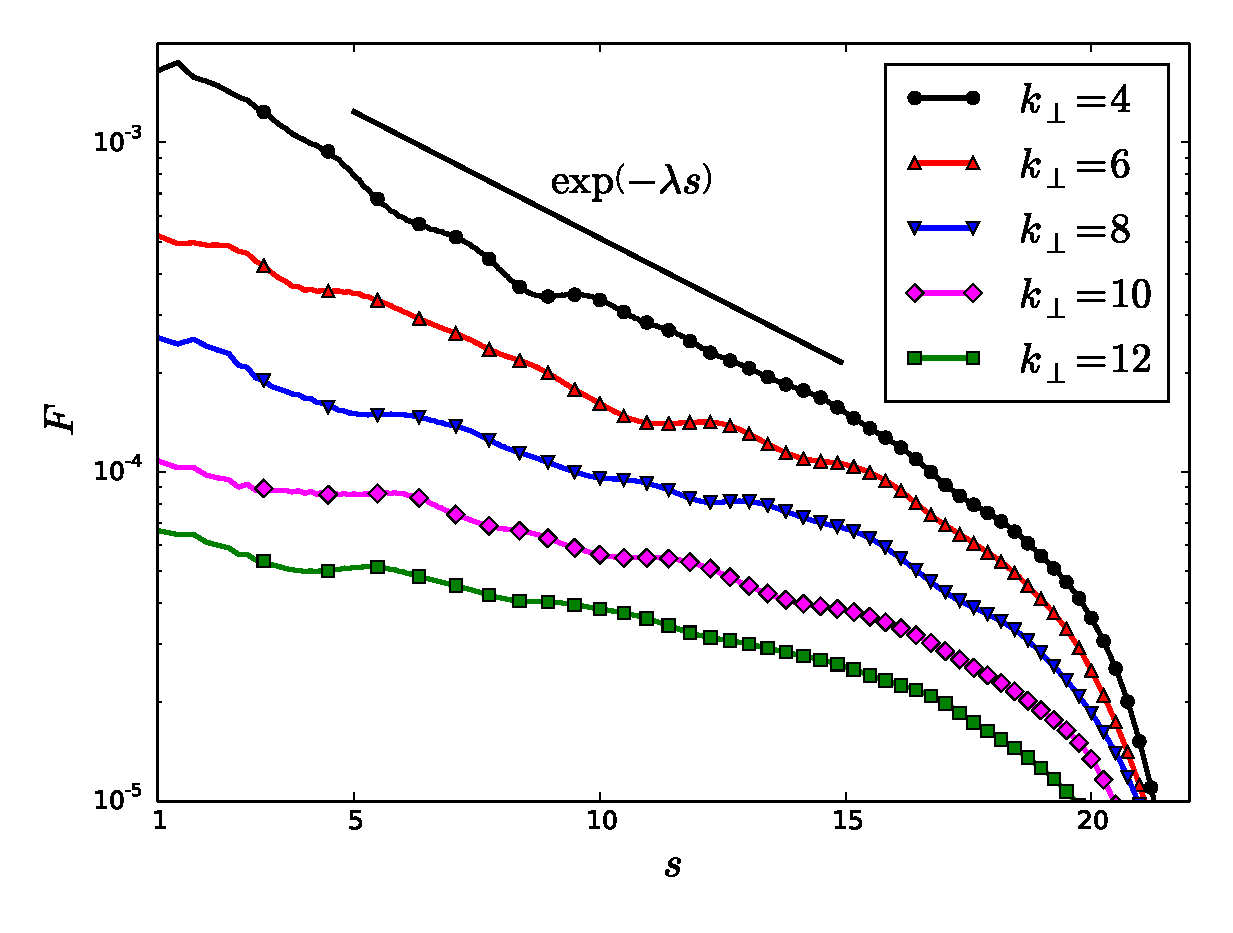
\includegraphics[width=14.8cm]{figs/phmixnl/M900_kz2_vss.eps}
%        \caption{Spectrum vs $s$ for parameters $\tauc
%        \simeq 1.5$, $s_c \simeq 21.3$, $k_{\perp, \eta} = 17.4$, $\kpar=2$. The spectrum
%        decays exponentially in $s$ at a
%        rate $\lambda\lt(k_\perp,\kpar\rt)$ for $\kpar\leq C_K k_\perp$.} 
%        \label{phmixnl:fig:1dsspec}
%    \end{center}
%    \end{figure}
%
%    \begin{figure}
%    \begin{center}
%        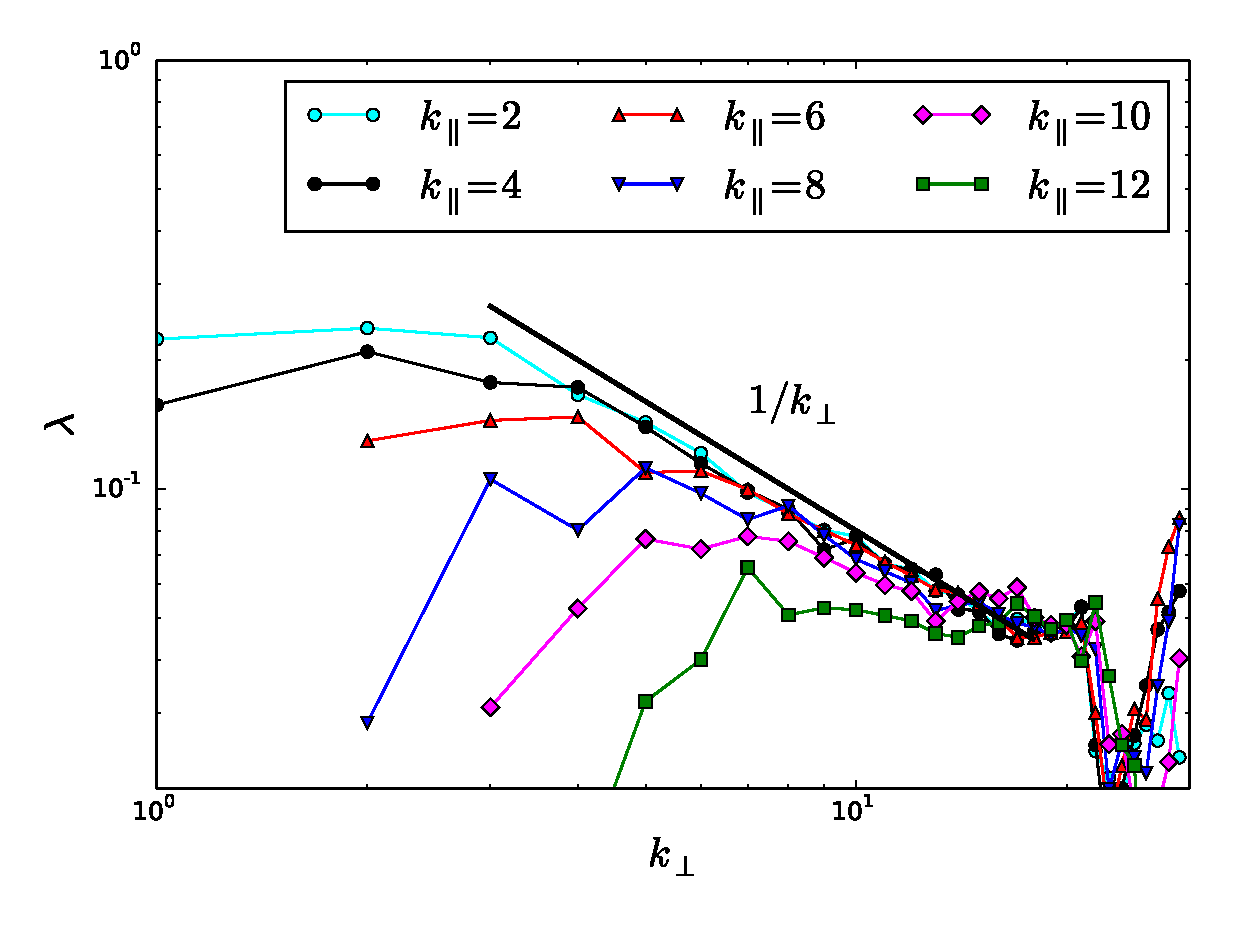
\includegraphics[width=14.8cm]{figs/phmixnl/M900_lambda_vskp.eps}
%        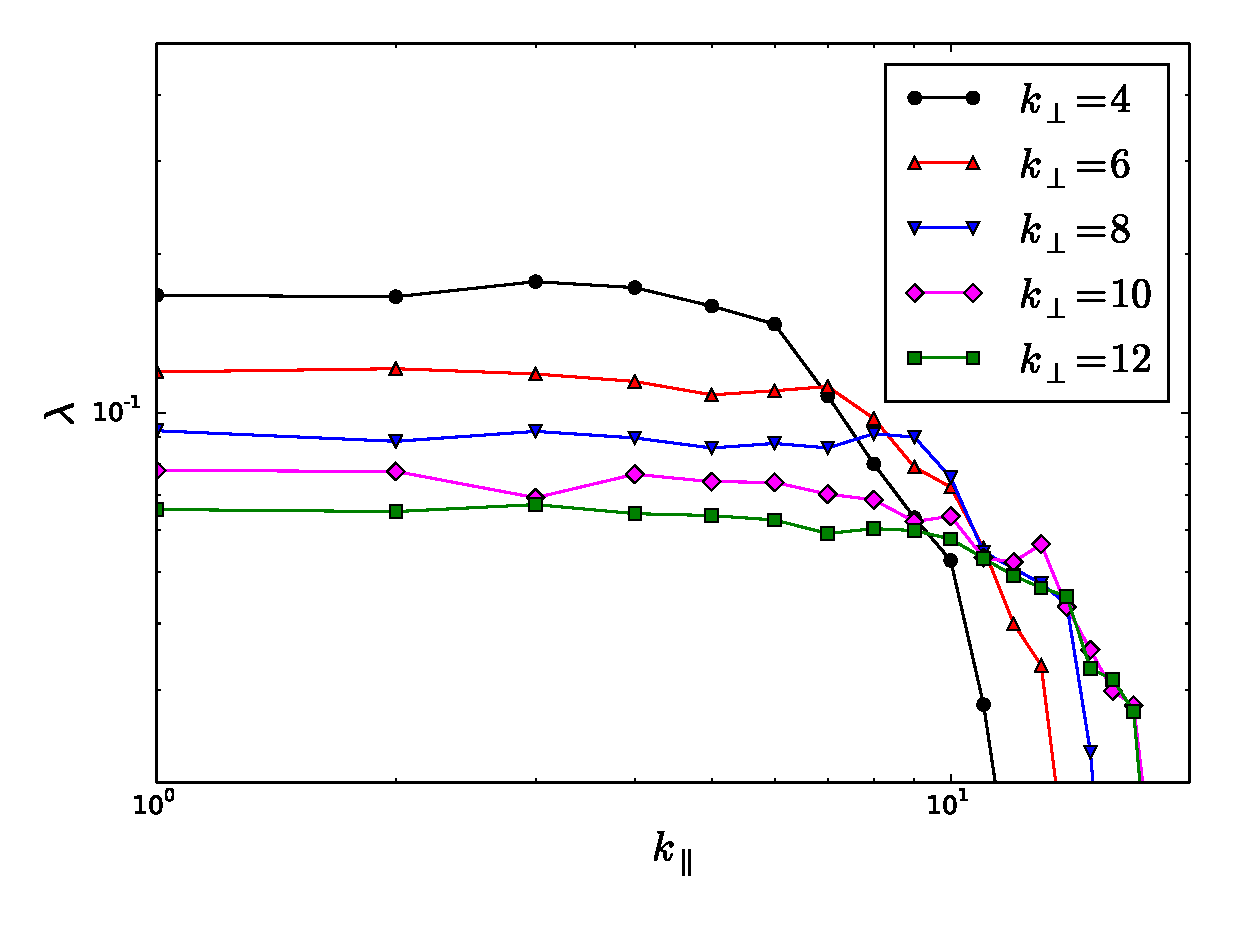
\includegraphics[width=14.8cm]{figs/phmixnl/M900_lambda_vskz.eps}
%        \caption{The decay rate $\lambda$ (see \figref{phmixnl:fig:1dsspec}) is independent of
%        $\kpar$, and is inversely proportional to $k_\perp$.}
%        \label{phmixnl:fig:1dsspec:lambda}
%    \end{center}
%    \end{figure}
%
%    The $s$ spectrum for $\kpar^3~\leq~\tauc~k_\perp^2~s_c$ decays exponentially at a rate
%    inversely proportional to $k_\perp$ and independent of $\kpar$ (see 
%    \figsand{phmixnl:fig:1dsspec}{phmixnl:fig:1dsspec:lambda}). For $\kpar~\geq~C_K k_\perp$, the $s$
%    spectrum is constant (see \figref{phmixnl:fig:1dsspec:2}).
%
%    \begin{figure}
%    \begin{center}
%        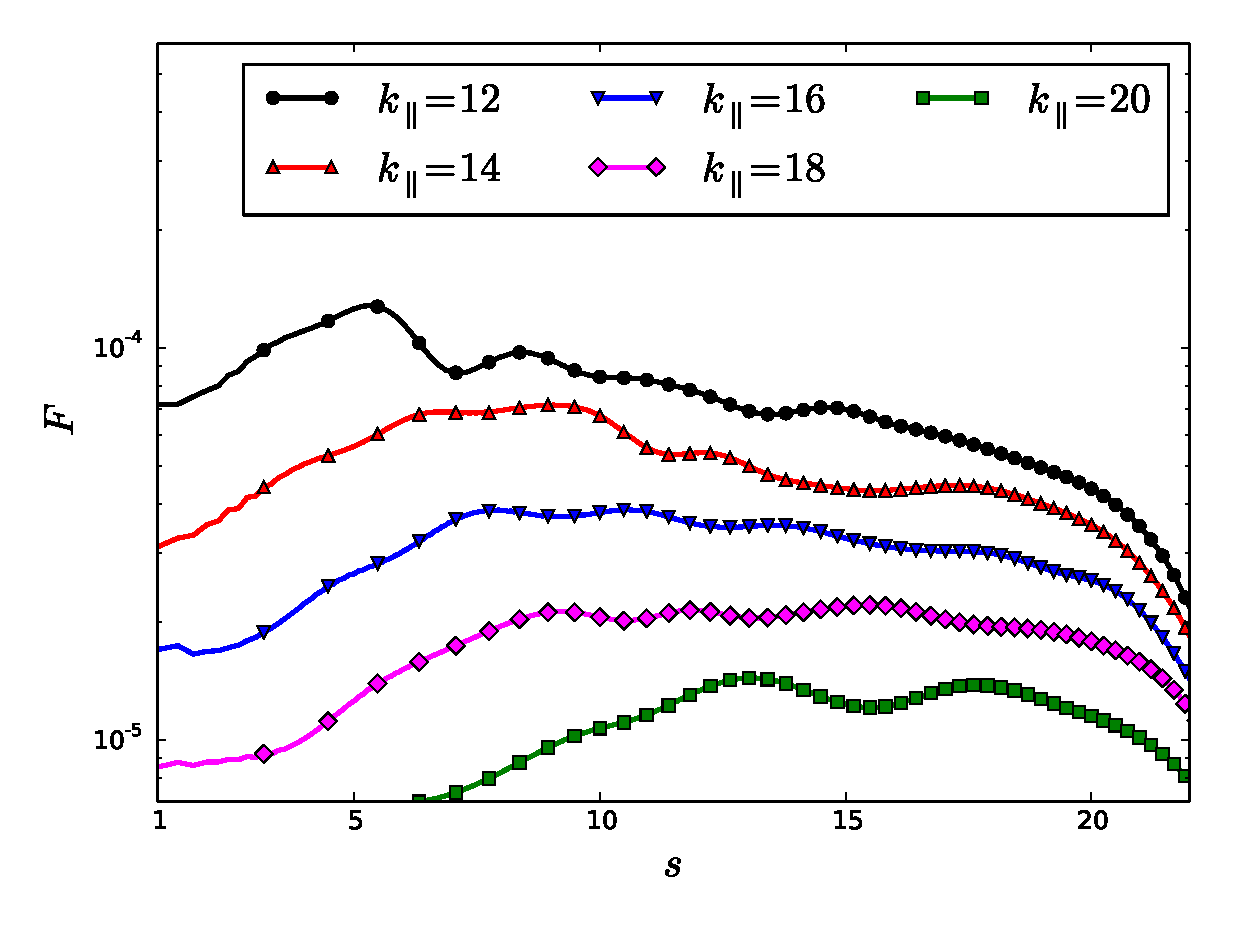
\includegraphics[width=14.8cm]{figs/phmixnl/M900_kp6_vss.eps}
%        \caption{Spectrum vs $s$ for parameters $\pu
%        \simeq 1.5$, $s_c \simeq 21.3$, $k_{\perp, \eta} = 17.4$, $k_\perp=6$. After an
%        initial ``transient", the spectrum is constant in $s$ for $\kpar\geq C_K k_\perp$.} 
%        \label{phmixnl:fig:1dsspec:2}
%    \end{center}
%    \end{figure}
%
    
%    This comes about as a
%    result of the competition between linear phase-mixing and the nonlinear turbulent
%    cascade.  Phase-mixing tries to drive the system towards a constant-in-$s$ spectrum
%    \cite{watanabe04, zocco11, hatch13, kanekar14a} on
%    an inverse timescale proportional to $\kpar\vth\sim~C_K~k_\perp\vth$, while the
%    nonlinear cascade transfers energy to large $\mb{k}$ at a rate $\pu$, attempting to
%    prevent any flux to high $s$; which results in the observed spectrum $\Fsk\sim\exp\lt(-\pu
%    s/\lt(C_K k_\perp \vth\rt)\rt)$.  For $\kpar~\geq~C_K k_\perp$,
%    the system is seen to approach a constant-in-$s$ spectrum (see
%    \figref{phmixnl:fig:1dsspec:3}).   

%\subsection{Flux in Hermite space}
%
%    To understand the numerically observed spectra from the previous section, we derive an equation for the spectrum
%    $\Fsk~=~\sqrt{m}k_\perp|\tgmk|^2$ by adding $``+"$
%    and $``-"$ equations in \eqref{phmixnl:eq:Fskpm} to obtain,
%    \bea
%        \pd{\Fsk}{t} + \pd{\Gsk}{s} + 2 \nu s^2 \Fsk + 2 \eta k_\perp^2 \Fsk =  \nonumber \\
%        \textit{Nonlinear terms}.
%        \label{phmixnl:eq:Fsk}
%    \eea
%    The second term on the left hand side of \eqref{phmixnl:eq:Fsk} describes the flux of energy to higher
%    Hermite moments; ignoring this term is equivalent to taking the fluid limit.
%    Interestingly, the spatial spectra observed in the previous section are same as
%    that for the fluid passive scalar: $\Fsk~\propto~k_\perp/\lt(\kpar^2 + C_K^2
%    k_\perp^2\rt)^{3/2}$. This suggests a constant flux steady state solution.
%    
%    \begin{figure}
%    \begin{center}
%        \includegraphics[width=14.8cm]{figs/phmixnl/M36_exsupp_m1_vskpkz.eps}
%        \includegraphics[width=14.8cm]{figs/phmixnl/M100_exsupp_m1_vskpkz.eps}
%        \caption{Normalized flux of free energy in Hermite space
%        $\Gsk/\lt(\sqrt{2}|\kpar|\vth \Fsk\rt)$ vs $k_\perp, \kpar$ at $s=1$ for
%        parameters $\pu \simeq 1.5$, $k_{\perp, \eta} = 17.4$. The top figure corresponds
%        to $s_c \sim 4.7$, and the bottom figure $s_c \sim 7.6$. Phase-mixing is nearly
%        completely suppressed in the region given by
%        $\kpar^3 \leq \pu k_\perp^2 |s_c-s|$.}
%    \label{phmixnl:fig:supp1} 
%    \end{center}
%    \end{figure}
%    \begin{figure}
%    \begin{center}
%        \includegraphics[width=14.8cm]{figs/phmixnl/M400_exsupp_m1_vskpkz.eps}
%        \includegraphics[width=14.8cm]{figs/phmixnl/M900_exsupp_m1_vskpkz.eps}
%        \caption{Normalized flux of free energy in Hermite space
%        $\Gsk/\lt(\sqrt{2}|\kpar|\vth \Fsk\rt)$ vs $k_\perp, \kpar$ at $s=1$ for
%        parameters $\pu \simeq 1.5$, $k_{\perp, \eta} = 17.4$. The top figure corresponds
%        to $s_c \sim 14.2$, and the bottom figure $s_c \sim 21.3$. Phase-mixing is nearly
%        completely suppressed in the region given by
%        $\kpar^3 \leq k_\perp^2 |s_c-s|$.}
%        \label{phmixnl:fig:supp2}
%    \end{center}
%    \end{figure}
%    \begin{figure}
%    \begin{center}
%        \includegraphics[width=14.8cm]{figs/phmixnl/M900_fpm_m1_vskpkz.eps}
%        \caption{Spectrum $\Fsk^\pm$ at $s=1$ vs $k_\perp, \kpar$ for parameters $\pu
%        \simeq 1.5$, $s_c \simeq 17.5$, $k_{\perp, \eta} = 17.4$. The phase-unmixing
%        spectrum $\Fsk^-$ is plotted on the left, whereas the phase-mixing spectrum
%        $\Fsk^+$ is plotted on the right.
%        The two components nearly cancel eachother in the trianglular region given by
%        $\kpar^3 \leq \pu k_\perp^2 s_c$, resulting in nearly zero net flux into Hermite space.} 
%        \label{phmixnl:fig:fpm:kpkzspec}
%    \end{center}
%    \end{figure}
%
%    \begin{figure}
%    \begin{center}
%        \includegraphics[width=14.8cm]{figs/phmixnl/N64_coll_m4kp12_vskz.eps}
%        \includegraphics[width=14.8cm]{figs/phmixnl/N64_coll_m49kp12_vskz.eps}
%        \caption{Spectrum $\Fsk^\pm$ vs $\kpar$ at $k_\perp=12$, for two different
%        collisionalities. The top plot is for $s=2$, whereas the bottom plot is for $s=7$.
%        For $s=2$, the two spectra nearly coincide proving convergence. However, for
%        $s=7$, there is substantially less energy in the phase-unmixing mode for the
%        collisional case as compared to the collisionless case. Collisional effects also
%        modify the $\kpar$ spectrum, since the solution is no longer the zero-flux
%        solution.}
%        \label{phmixnl:fig:coll:vskz}
%    \end{center}
%    \end{figure}
%
%    Net flux through the first Hermite moment is observed to be nearly zero for
%    wavenumbers in the range $\kpar^3 \leq \pu k_\perp^2 s_c$ (see
%    \figsand{phmixnl:fig:supp1}{phmixnl:fig:supp2}). In this region, the free energy is nearly
%    equally partitioned between the phase-mixing and the phase-unmixing components, 
%     (see \figref{phmixnl:fig:fpm:kpkzspec}),  demonstrating that the stochastic plasma echo is responsible
%     for the zero flux solution. 
%
%    \begin{figure}
%    \begin{center}
%        \includegraphics[width=14.8cm]{figs/phmixnl/M900_exsupp_kp8_vsskz.eps}
%        \includegraphics[width=14.8cm]{figs/phmixnl/M900_exsupp_kz8_vsskp.eps}
%        \caption{Normalized flux of free energy in Hermite space
%        $\Gsk/\lt(\sqrt{2}|\kpar|\vth \Fsk\rt)$ for parameters $\pu \simeq 1.5$,
%        $k_{\perp, \eta} = 17.4$, $s_c \sim 21.3$, plotted vs $s-\kpar$ at $k_\perp=8$ in
%        the top plot, and vs $s-k_\perp$ at $\kpar=8$ in the bottom plot. The suppressed
%        region is given by $\kpar^3 \leq \pu k_\perp^2 |s_c - s|$.}
%        \label{phmixnl:fig:supp3}
%    \end{center}
%    \end{figure}
%     
%     The extent of the suppressed region is
%     determined by the collisionality of the system. Collisional dissipation
%    extracts energy from a phase-mixing mode before it can couple to an phase-unmixing
%    mode. This sets an upper bound in $\kpar$, given by $k_{\parallel, c} \sim
%    \lt(\pu k_\perp^2 \lt|s_c-s\rt|\rt)^{1/3}$, beyond which there is no 
%    energy in the phase-unmixing modes, resulting in finite non-zero flux into Hermite
%    space (see \figref{phmixnl:fig:supp3}). 
%    
%    This deviation from the zero-flux solution can also be gleaned from the parallel
%    spectra plotted in \figref{phmixnl:fig:coll:vskz}---parallel spectrum for the more
%    collisional system is not the same as that for the fluid passive scalar, this is also
%    the part of phase space where phase-mixing is not suppressed.
%     %This can also be diagnosed by looking at
%     %the behavior of the system at different values of $s$ in the same simulation; since
%     %the dynamics in the Hermite space is universal (see \eqref{phmixnl:eq:gmeq}), looking at the
%     %spectra and suppression at a higher value of $s$ is roughly equivalent to studying a
%     %a more collisional system.
%
%
%    %\begin{figure*}
%    %\begin{center}
%    %    \includegraphics[width=18cm]{figs/phmixnl/M900_mat_vss.eps}
%    %    \caption{Spectrum vs $s$ for parameters $\pu
%    %    \simeq 1.5$, $s_c \simeq 17.5$, $k_{\perp, \eta} = 17.4$, for multiple values of
%    %    $k_\perp, \kpar$. The numbers in the top right corner of each little plot denote
%    %    the $(k_\perp, \kpar)$ values. The dotted line plots $\exp(-\pu s/(2 k_\perp
%    %    \vth)$.} 
%    %    \label{phmixnl:fig:sspec:mat}
%    %\end{center}
%    %\end{figure*}
%
%    
%
%%    The zero-flux solution discussed above is true for values of $s$ where collisions can
%%    be safely ignored. For larger $s$, collisional dissipation
%%    extracts energy from a phase-mixing mode before it can couple to an phase-unmixing
%%    mode. This effectively sets an upper bound in $\kpar$ beyond which there is no 
%%    phase-unmixing mode, resulting in finite non-zero
%%    flux into Hermite space. This deviation from the zero-flux solution can be seen from the parallel spectra plotted in \figref{phmixnl:fig:coll:vskz}.
%%
%    \begin{figure}
%    \begin{center}
%        \includegraphics[width=14.8cm]{figs/phmixnl/M900_visc_kp4kz4_vss.eps}
%        \includegraphics[width=14.8cm]{figs/phmixnl/M900_visc_kp8kz4_vss.eps}
%        \caption{Spectrum $\Fsk$ vs $s$ at $k_\perp=12$, for two different
%        viscosities. The top plot is for $k_\perp=4, \kpar=4$, whereas the bottom plot
%        is for $k_\perp=8, \kpar=4$.
%        For $k_\perp=4, \kpar=4$, the two spectra nearly coincide proving convergence. However, for
%        $k_\perp=8, \kpar=4$, the spectrum for the viscous case is steeper.}
%        \label{phmixnl:fig:visc:vss}
%    \end{center}
%    \end{figure}
%
%    We discussed the effect of collisional dissipation on the steady-state solution of our
%    model. Finite viscous effects modify the solution as well---
%    viscosity sets a cutoff in $k_\perp$, which in turn sets a cutoff in $\kpar$; as a
%    result the $s$ spectrum for modes close to the viscous cutoff have a steeper $s$
%    spectrum as shown in \figref{phmixnl:fig:visc:vss}.
    
\section{Conclusions and discussion}

    We demonstrated with a simplified model for kinetic passive scalar turbulence that
    Landau damping, or more generally phase mixing can be suppressed significantly in
    turbulent systems for a part of the phase space. Energy is scattered in the phase
    space such that the net flux to higher Hermite moments of the distribution
    function is reduced due to the stochastic plasma echo.
    We showed using direct numerical simulations that phase mixing is 
    suppressed significantly in the region $\kpar^3 \leq \pu k_\perp^{2/3} s_c$.
    Therefore, in the collisionless limit ($s_c \to \infty$), phase mixing would be suppressed
    in the whole inertial range.
    Perpendicular and parallel spectra were shown to be the same as fluid spectra in the
    suppressed region.
    The suppression of Landau damping by the stochastic plasma echo helps explain why
    power law energy spectra survive at scales where fluctuations are expected to be
    strongly damped, by linear theory.

    Here, we conclude our
    treatment of the kinetic passive scalar (chapters \ref{chap:phmixlin}, \ref{chap:pp0}
    and \ref{chap:phmixnl}), and give a summarized list of our results so
    far:
    \begin{itemize}
        \item We analytically derived the fluctuation-dissipation relations in the linear
        limit for the kinetic passive scalar.

        \item We constructed an analytical framework to diagnose the efficiency of phase
        mixing by considering the flow of energy in the Hermite space. Within this
        framework, we proved that
        in the linear limit, the steady state solution to the system is a constant-flux
        solution, and that the energy solely flows from small to large Hermite moments for
        large values of $\sqrt{m}$.

        \item When the passive scalar is being mixed by a 2D velocity field,
        the spectrum in the Hermite space is exponentially attenuated in the strong turbulence regime, and the
        behavior of the kinetic system is essentially fluid-like. This is a result of the
        energy in the passive scalar being swept up to small spatial scales by the
        advecting velocity field, before it can phase mix.

        \item On the other hand, if the scalar is being mixed by a 3D velocity, there is a stochastic analog of the plasma
        echo which suppresses the 
        efficiency of phase mixing in a part of the phase space, the
        extent of which is determined by the collisionality of the system, and the
        amplitude of the advecting velocity. 
    \end{itemize}

    In the next chapter, we use these ideas, and the diagnostic tools developed here to study the compressive
    fluctuations cascade in the kinetic reduced MHD limit.
    
